\documentclass[11pt, conference]{IEEEtran}
\IEEEoverridecommandlockouts

\usepackage{cite}
\usepackage{amsmath,amssymb,amsfonts}
\usepackage{algorithmic}
\usepackage{graphicx}
\usepackage{textcomp}
\usepackage{xcolor}
\usepackage{kotex}
\usepackage{booktabs}
\usepackage{tabularx}
\usepackage{supertabular,booktabs}
\usepackage{adjustbox}
\usepackage{enumitem}
\usepackage{romannum}
\usepackage{makecell}
\usepackage{multirow}
\usepackage{hyperref}
\usepackage{graphics}
\usepackage{subfigure}
\usepackage{float}
\hbadness=99999  % or any number >=10000
\vbadness=99999  % or any number >=10000
\hfuzz=20pt
\def\BibTeX{{\rm B\kern-.05em{\sc i\kern-.025em b}\kern-.08em T\kern-.1667em\lower.7ex\hbox{E}\kern-.125emX}}
\begin{document}

% function
% add new image with full width
% usage:
% \addImageFull{
%     imgs/specification/login_page.png
% }{
%     description to image
% }
\newcommand{\addImageFull}[2]{
    \begin{figure}[ht]
        \begin{center}
            \includegraphics[width=8cm]{#1}
            \caption{#2} % description to image
            \renewcommand{\thefigure}{\thesubsection.\arabic{figure}}
        \end{center}
    \end{figure}
}

% function
% add new image with specific size
% usage:
% \addImageSize{
%     5cm
% }{
%     imgs/specification/login_page.png
% }{
%     description to image
% }
\newcommand{\addImageSize}[3]{
    \begin{figure}[ht]
        \begin{center}
            \includegraphics[width={#1}]{#2}
            \caption{#3} % description to image
            \renewcommand{\thefigure}{\thesubsection.\arabic{figure}}
        \end{center}
    \end{figure}
}

\setcounter{figure}{0}

\title{IOT Home Heroes\\
\small{Seamless home automation based on posture/position detection\\}
}

\makeatletter
\newcommand{\linebreakand}{
  \end{@IEEEauthorhalign}
  \hfill\mbox{}\par
  \mbox{}\hfill\begin{@IEEEauthorhalign}
}
\makeatother

\author{
  \IEEEauthorblockN{Jo Taesik}
  \IEEEauthorblockA{\textit{dept. of Information Systems} \\
    \textit{Hanyang University}\\
    Seoul, Korea\\
    r4pidstart@hanyang.ac.kr}
  \and
  \IEEEauthorblockN{Kwon Jongin}
  \IEEEauthorblockA{\textit{dept. of Information Systems} \\
    \textit{Hanyang University}\\
    Seoul, Korea \\
    whddlswhdaud@naver.com}
  \and
  \IEEEauthorblockN{Bae Hyojeong}
  \IEEEauthorblockA{\textit{dept. of Information Systems} \\
    \textit{Hanyang University}\\
    Seoul, Korea \\
    bhj09270@hanyang.ac.kr}
  \linebreakand % <------------- \and with a line-break
  \IEEEauthorblockN{Lee Hyunsuk}
  \IEEEauthorblockA{\textit{dept. of Information Systems} \\
    \textit{Hanyang University}\\
    Seoul, Korea \\
    leehyunsuk2000@gmail.com}
  \and
  \IEEEauthorblockN{Nan Haixu}
  \IEEEauthorblockA{\textit{dept. of Information Systems} \\
    \textit{Hanyang University}\\
    China, Guangzhou \\
    what-is-my-id@naver.com}
}

\maketitle
\begin{abstract}
\textit{With the recent surge in fascination with home automation, numerous companies are investigating strategies to facilitate the unified management of connected devices. A few of these techniques comprise verbal requests to a service for a particular action or the activation of a specific action when motion is sensed by designated sensors. Nevertheless, these approaches possess limitations that necessitate users to execute certain requests or actions that they would not typically perform to direct their devices. Devices also do not enable the full comprehension of the user's intentions. These restrictions do not meet the requirements of users who seek to construct home automation that can naturally recognize their intentions and respond correspondingly. Our proposal is to offer a service permitting users to initiate particular actions by way of genuine, intentional behavior that feels natural. This service offers a platform to assimilate and manage devices via the Matter protocol. On this platform, users can determine which actions are activated based on users interactions with certain objects in specific locations. By using IP cameras connected to the platform, OpenPose, Library for pose estimation assesses the user's posture, labelling it as sitting, lying down, standing, and more. By recognizing the posture of the user and specific objects, pre-defined actions are triggered. With this service, User can advance beyond traditional home automation to create a system that operates by comprehending user's intents with greater precision.\\}
% 최근 홈 오토메이션에 대한 관심이 높아짐에 따라, 여러 기업들은 연결된 기기를 통합적으로 간편하게 제어하기 위한 방법을 연구하고 있습니다. 음성으로 서비스를 호출하여 특정 액션을 요청한다던지, 특정 센서에 움직임이 감지되면 특정 액션이 트리거되는 등의 방법이 존재합니다. 그러나 이러한 방법들에는 한계가 존재합니다. 사용자로 하여금 기기를 제어하기 위해서가 아니라면 하지 않았을,  특정한 호출이나 동작을 강제합니다. 또한 사용자가 진정으로 무엇을 의도하는지 알 수 없다는 점도 있습니다. 이러한 한계는 자연스럽게 내 의도를 파악하여 그에 맞는 행동을 하는 홈 오토메이션을 구축하길 원하는 사용자들의 니즈를 충족시킬 수 없습니다. 그래서 우리는 사용자들이 부자연스럽지 않은, 의도가 담긴 자연스러운 동작을 통해 특정 액션을 트리거할 수 있는 서비스를 제안합니다. 이 서비스는 Matter 프로토콜을 이용해 기기들을 통합하고, 관리할 수 있는 플랫폼을 제공합니다. 이 플랫폼에서, 유저는 어느 위치의 어떤 사물에서 어떤 동작을 취하는지에 따라 어떤 액션이 트리거될 지를 설정할 수 있습니다. 이 플랫폼에 연결된 카메라를 이용해, openpose가 유저의 자세를 추정합니다. 이때 앉거나, 눕거나, 일어나는 등으로 유저의 자세를 분류합니다. 이런 방법으로 지정된 사물에서 설정해놓은 자세를 취하는 것을 인식하면 미리 지정된 액션을 트리거합니다. 이 서비스를 이용해 유저는 기존의 홈 오토메이션보다 한 단계 앞서 작동하고, 유저의 의도를 더욱 더 잘 파악하여 동작하는 홈 오토메이션을 완성할 수 있습니다.
\end{abstract}

\begin{IEEEkeywords}
home automation, IOT, Matter, pose estimation, OpenPose \\\\\\\\
\end{IEEEkeywords}

\large{Role Assignments}
\begin{table}[H]
\center
\begin{tabular}{m{1.4cm} m{1.5cm} m{4cm}}
\toprule
Roles & Name & Task description \& etc.\\
\midrule
User & Bae Hyojeong & He expects that he will be able to use them to make his life easier by operating IOT devices, However, He is hesitant because of the negative reviews from people who have already used them, or he is afraid that it will be too difficult to install and set them up. \\\\
Customer & Kwon Jongin & Created a product that can be controlled using IOT, but consumers rarely use the feature because it's not as convenient as expected. He is looking for ways to make his product more convenient to use in order to get consumers to use product. \\\\
Software developer & Lee Hyunsuk, Nan Haixu & Designs and implements a solution to a given problem. Able to troubleshoot problems that may arise during development and complete assigned tasks within a given timeframe. \\\\
Development manager & Jo Taesik & Breaking down a given task into solvable problems and distributing them appropriately among team members. They also coordinate schedules to ensure that tasks are completed within a given timeframe. \\
\bottomrule
\end{tabular}
\end{table}
\newpage

\section{\Large{Introduction}}
% \begin{enumerate}[label=\arabic*]
%%%%%%%%%%%%%%%%%%%%%%%%%%%%%%%%%%%%%%%%%%%%
\subsection {\large{Motivation}}
The IOT market has been growing rapidly in recent years. According to IOT Analytics, the IOT device market, which was valued at \$120 billion in 2019, is growing at a staggering rate, reaching \$100 billion in the first quarter of 2023. This market is also expected to grow at a CAGR of 20\% in the future. According to the same organization, there are currently an estimated 14.4 billion connected IOT devices, which is also expected to grow at a CAGR of 16\%. \\

\begin{figure}[ht]
    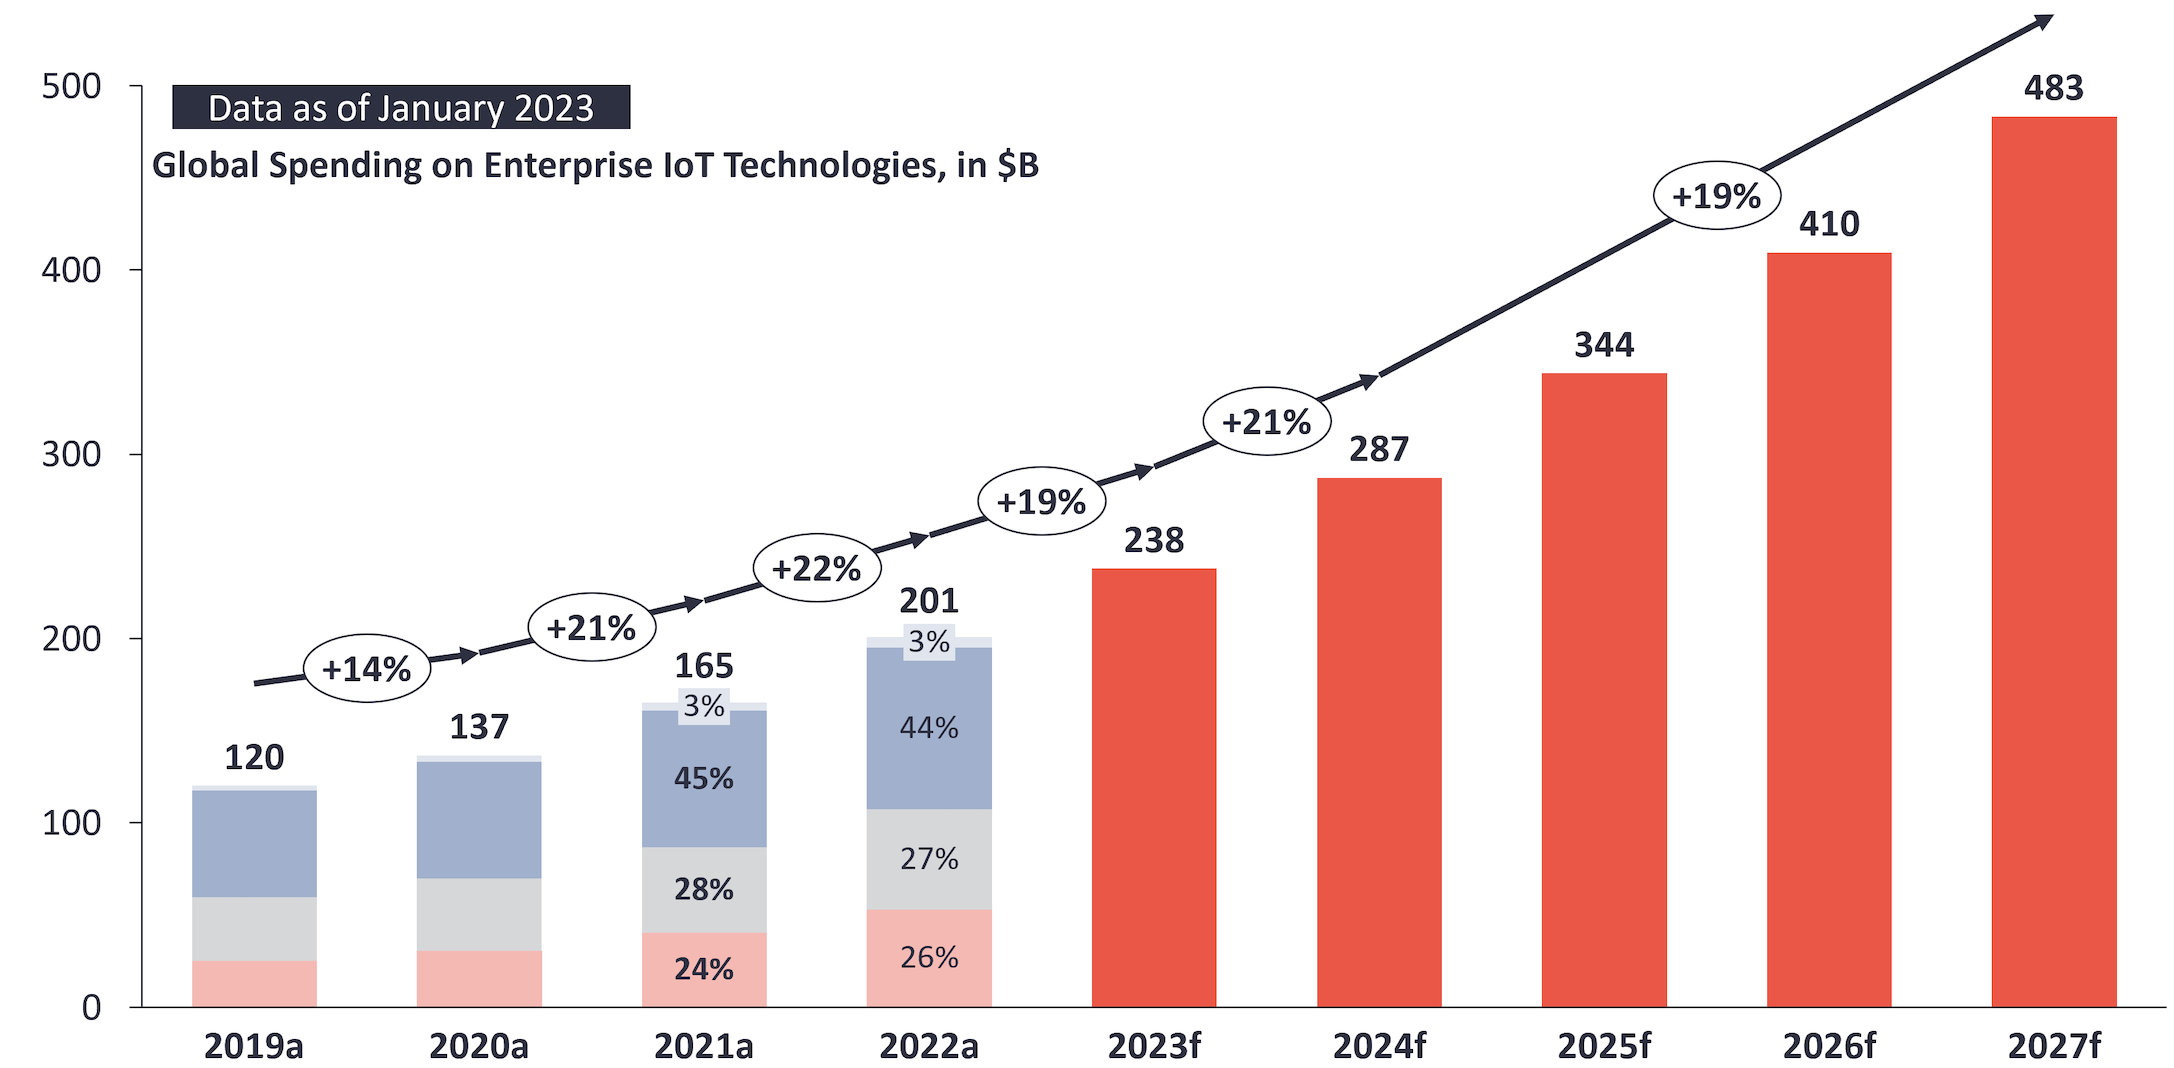
\includegraphics[width=8cm]{imgs/introduction/iot_market_growing.png}
    \caption{Growing IOT market}
    \renewcommand{\thefigure}{\thesubsection.\arabic{figure}}
\end{figure}

In response to this market growth, many electronics manufacturers have begun to include IOT-related technologies in their products, ranging from passive technologies that allow you to control your device through an application on your phone, to technologies that allow you to control multiple devices with a single device in conjunction with devices such as smart speakers, to more advanced technologies such as air quality sensors and motion recognition sensors that allow you to operate your device automatically without human command. \\

Consumer interest in IOT technologies is on the rise, and according to OpenSurvey, the number of consumers who own a home appliance with these technologies has grown from 29.5\% in 2022 to 48.3\% in 2023, an increase of 18.8 percentage points over the previous year.\cite{iot-market-size} \\\\

\begin{figure}[ht]
    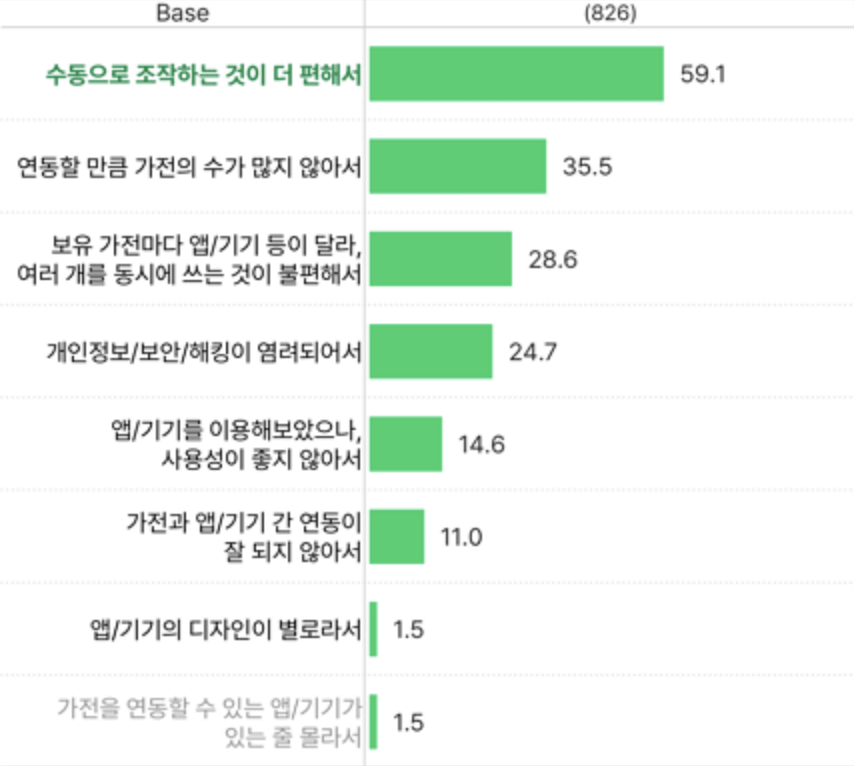
\includegraphics[width=8cm]{imgs/introduction/reason_why_not_use_iot.png}
    \caption{Reasons for not using IOT devices}
    \renewcommand{\thefigure}{\thesubsection.\arabic{figure}}
\end{figure}

However, consumers who have tried these technologies are often disappointed with devices that don't deliver on their pre-purchase expectations and stop using them. There are a few main reasons why this happens. According to OpenSurvey, these are the top reasons consumers have IOT devices but don't use them. \cite{iot-opensurvey}\\
\begin{enumerate}
    \item They are more comfortable operating them manually (59.1\%)\\
    \item They have different apps/devices for each device they own and don't want to use multiple devices at the same time (28.6\%)\\
    \item They have tried the apps/devices but don't like the usability (14.6\%)\\
    \item The apps/devices don't work well with their devices (11.0\%)\\
\end{enumerate}

We propose a platform to address the necessary issues for consumers to utilize IoT technologies. Our integrated IoT platform employs posture recognition to activate desired functions.\\\\

\newpage
%%%%%%%%%%%%%%%%%%%%%%%%%%%%%%%%%%%%%%%%%%%%
\subsection {\large{Problem Statement}}
\begin{enumerate}[label=\alph*]
    \item Uncomfortable Automation\\
          There is a gap between what users think home automation should be and what current platforms offer. Users assume that machines will interpret their intentions and complete tasks without any input, but the reality is quite the opposite. The machines can only perform specific procedures that have already been entered, and they lack the ability to determine when those procedures should be executed. Currently, the sole means of inducing a machine to execute a task is through summoning a voice assistant with a designated command and directing it to execute a specific procedure. This hindrance fosters the belief that it is more convenient to manually operate a device than to avail oneself of automation. Consequently, users will avail themselves of IOT features only under highly restricted circumstances.\\

    \item Complexity of Use\\
          Currently, IOT devices from manufacturers and platforms can only be controlled through voice recognition. However, this method is too limited for users who desire a fully-fledged smart home. Third-party platforms exist for these users, which provide more detailed and advanced features. Although these platforms are not officially supported by the manufacturers, users who encounter problems must solve them on their own. Connecting devices to the platform and building the server are required tasks. Additionally, these platforms these platforms describe their behavior in code, which means users have to get used to it. These factors increase complexity and may present a barrier to entry for the users.\\

    \item Security Concerns\\
          Devices that use a manufacturer's platform can pose security risks by sending all user and device information to the manufacturer's servers. This compromise exposes sensitive personal information and lifestyle details to potential exploitation. Additionally, it opens up the possibility for malicious actors to manipulate and misuse devices in the home remotely.\\

    \item Disjointed communication methods\\
          Numerous communication methods are utilized in IoT devices these days, encompassing traditional WiFi and Bluetooth as well as UWB, RFID, Zigbee, Z-WAVE, XBee, LoRa, SigFox, and many others. Device manufacturers have selected one or more communication methods to construct their devices, resulting in consumers being limited to devices that use a specific communication method based on the hub they utilize.\\

          \begin{figure}[ht]
              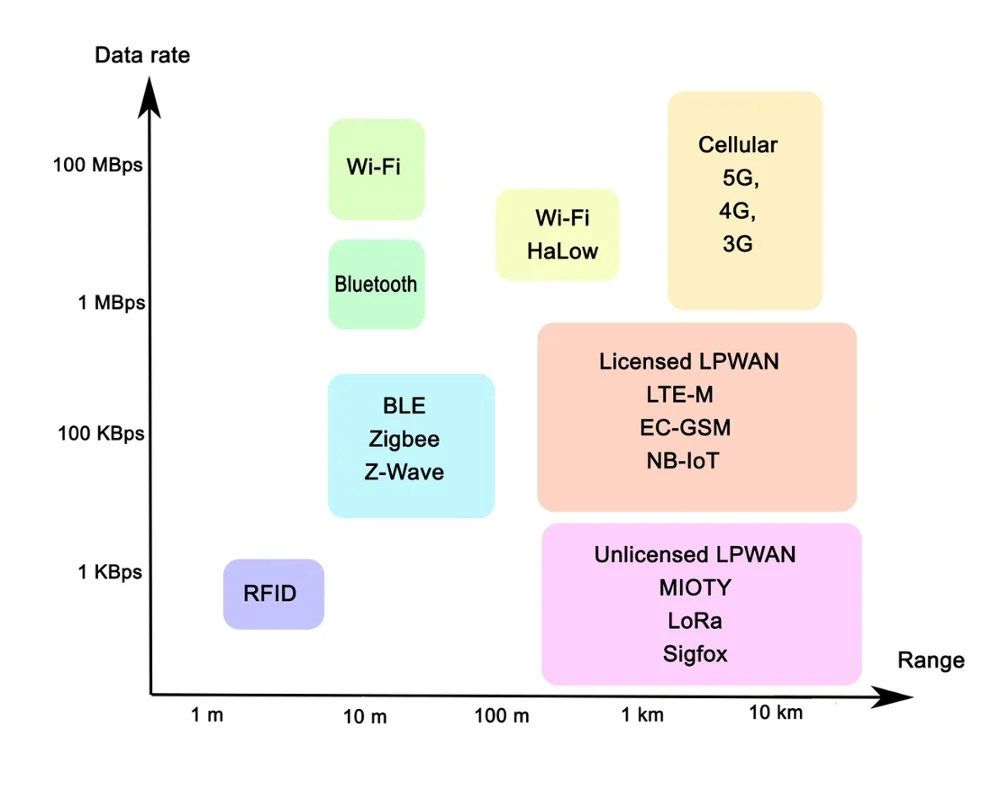
\includegraphics[width=7.5cm]{imgs/introduction/iot-protocols.png}
              \cite{iot-protocols}
              \caption{IOT protocols}
              \renewcommand{\thefigure}{\thesubsection.\arabic{figure}}
          \end{figure}

    \item Fragmented Platforms\\
          IOT device manufacturers maintain distinctive platforms and require navigating their platforms and hubs for using a specific device of a manufacturer. This limitation restricts the full functionality of devices to the manufacturer's designated platform, rendering interoperability difficult. Some manufacturer hubs do not allow devices from other manufacturers to connect, causing consumers to lean towards one manufacturer for their smart home devices and discouraging the use of products from different manufacturers at the same time. It also creates challenges when replacing a product line that is not made by a particular manufacturer, thus limiting consumer options.

\end{enumerate}
%%%%%%%%%%%%%%%%%%%%%%%%%%%%%%%%%%%%%%%%%%%%
\subsection {\large{Related Software}}
\begin{enumerate}[label=\alph*]
    \item Google Home\\
          \addImageSize{5cm}{imgs/introduction/home.png}{Google Home}\\
          This is a smart home platform offered by Google. It is compatible with a variety of devices, including lights, thermometers, speakers, and more. Additionally, it works with the Google Assistant, which allows you to check the status of your devices or control them. The same can be done through the accompanying application. Routines tailored to specific circumstances can be created and activated via voice commands. Easily add family members to share routines and jointly control devices. In addition to setting things up in the application, user can automate the details using YAML scripts.\\\\

    \item Apple Home\\
          \addImageSize{5cm}{imgs/introduction/homekit.png}{Apple Homekit}\\
          This is a smart home platform offered by Apple that is compatible with a variety of devices including lights, thermometers, and speakers, among others. It works with the Siri, which allows you to check the status of your devices or control them. The same can be done through the accompanying application. One can conveniently monitor device status via Control Center or widgets on other Apple devices. An Apple TV can also serve as a hub and automatically regulate devices based on circumstance, including weather, motion, or humidity. However, an Apple device is required.\\\\

    \item Samsung Smartthings\\
          \addImageSize{6cm}{imgs/introduction/smartthings.png}{Samsung Smartthings}\\
          This is a smart home platform offered by Samsung. This platform is compatible with a variety of devices, including lights, thermometers, and speakers. Users can access and manage device status via Bixby or the application. To take full advantage of the IOT capabilities of their Samsung home appliances, users need this platform. User can utilize their Samsung devices as sensors. Unlike platforms offered by other manufacturers, Smartthings is an open platform, allowing for connection of even unsanctioned products through various actions. The hub permits connection of third-party sensors and setup of automation routines.\\\\

    \item LG ThinQ\\
          \addImageSize{7cm}{imgs/introduction/thinq.png}{LG ThinQ}\\
          This is a smart home platform designed by LG that is necessary for full utilization of the IOT features of LG appliances. Users can receive notifications when their appliances finish their tasks, diagnose problems with their appliances, and schedule after-sales services. They can also integrate with Apple HomeKit to monitor or control their HomeKit-connected devices using this application.\\\\


    \item Home Assistant\\
          \addImageSize{7cm}{imgs/introduction/homeassistant.png}{Home Assistant}\\
          This is the sole mainstream smart home platform founded on open-source principles. The software can be installed and run on various hardware, including Raspberry Pi or Odroid. Devices with Home Assistant behave as hubs once the software is installed.\\

          \begin{figure}[ht]
              \begin{center}
                  \raggedleft
                  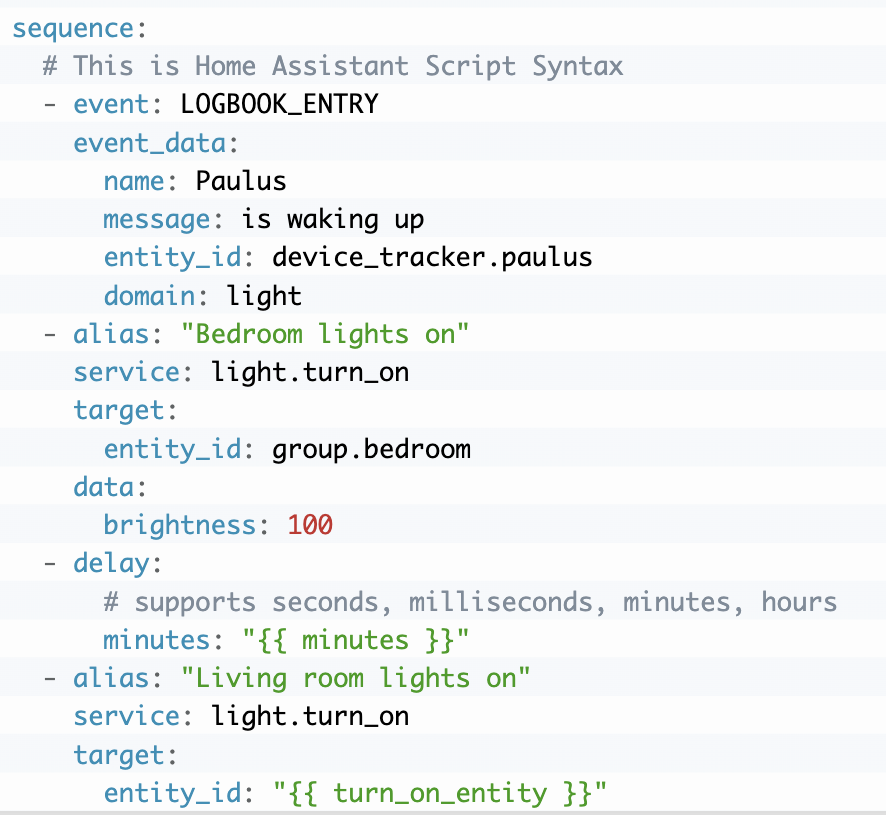
\includegraphics[width=8cm]{imgs/introduction/ha_script_example.png}
                  \caption{Home Assistant script example}
                  \renewcommand{\thefigure}{\thesubsection.\arabic{figure}}
              \end{center}
          \end{figure}

          It supports a diverse range of protocols and easily connects to devices unsupported by it through multiple actions. It is more difficult to configure than other platforms, but after mastering it, scripts can be utilized to access any data from linked devices and automate actions in numerous ways.\\


\end{enumerate}
\section{\Large{Requirement Analysis}}
\begin{enumerate}[label=\arabic*.]
    \item {\large{Login}}\\

          \begin{enumerate}[label*={\arabic*.},ref=\theenumi.\arabic*]
              \setlength{\itemindent}{0.5cm}
              \item The user must log in to their own account, which contains their personal information.\\

              \item This application should be customizable for homeowners, so user’s personal information need to be stored in his/her own account.\\

              \item If the user manages multiple devices, the information is required for connecting to several devices.\\

                    % \item User can add and remove devices he/she manages through QR code(It is also possible without the QR code).\\

              \item For the login process, user inputs their ID and password within the app.\\

              \item Alternatively, users can utilize an external ID, like a Google or Apple ID, to conveniently sign in without having to register.\\

              \item ID must include at least 5 English or English and numbers both.\\

              \item Password must include at least 4 uppercase letters, special characters, and numbers.\\

              \item When the user sign up, he/she sets a username.\\

              \item Username must be unique: Each user must have a unique username within the system to ensure proper identification and to prevent any confusion or conflicts.\\
          \end{enumerate}

    \item {\large{Logs and Statistics}}\\
          \begin{enumerate}[label*={\arabic*.},ref=\theenumi.\arabic*]
              \setlength{\itemindent}{0.5cm}
              \item The application records user activities, including events such as trigger activation time, routine name, and user's location. \\

              \item It maintains device interaction logs, tracking device status changes, usage patterns, and scheduled events or automations triggered by the user. \\


              \item User behavior, preferences, and usage patterns are monitored to enhance this service. \\

              \item To achieve this, it stores a history of device status data, allowing users to review past device activities.\\
          \end{enumerate}


    \item {\large{Dashboard}}\\
          \begin{enumerate}[label*={\arabic*.}]
              \item {\large{Device Connection}}\\
                    \begin{enumerate}[label*={\arabic*.},ref=\theenumi.\arabic*]
                        \setlength{\itemindent}{0.5cm}
                        \item This application provide users with the ability to connect devices, including device pairing and disconnection.\\
                        \item Implement a QR code-based device connection method, allowing users to easily pair devices by scanning QR codes.\\
                        \item Offer an alternative method for connecting to devices without the use of QR codes, providing flexibility in device pairing.\\
                    \end{enumerate}

              \item {\large{Device Status Check}}\\
                    \begin{enumerate}[label*={\arabic*.},ref=\theenumi.\arabic*]
                        \setlength{\itemindent}{0.5cm}
                        \item This application implements a system to log and monitor the status of connected devices, including health assessments and connectivity information.\\
                        \item It should create and maintain records of status check activities, recording when these checks were performed, the specific devices involved, and the results indicating device operational status or reported issues.\\
                    \end{enumerate}

              \item {\large{Device Control}}\\
                    \begin{enumerate}[label*={\arabic*.},ref=\theenumi.\arabic*]
                        \setlength{\itemindent}{0.5cm}
                        \item  Implement the ability for users to manually control devices, including actions like turning devices on or off, adjusting settings, and triggering automation sequences.\\
                        \item Establish a logging system to track these control actions, capturing the date and time of each action, specifying the devices affected, and identifying the responsible user for each action.\\
                        \item Provide users with the capability to view the live feed or recorded content from connected devices like home security cameras.\\
                        \item Allow users to rename devices for personalization.\\
                        \item Enable users to delete devices when they are no longer needed or want to remove them from their account.\\
                    \end{enumerate}
          \end{enumerate}

    \item {\large{Routine Managemant}}\\
          \begin{enumerate}[label*={\arabic*.}]
              \item {\large{Trigger Settings}}\\
                    \begin{enumerate}[label*={\alph*.},ref=\theenumi.\arabic*]
                        \setlength{\itemindent}{0.5cm}

                        \item {\large{Sound Trigger}}\\
                              \begin{enumerate}[label*={\arabic*.},ref=\theenumi.\arabic*]
                                  \setlength{\itemindent}{0.5cm}
                                  \item Users can set conditions based on the intensity of sound to trigger accessories or scenes.\\
                                  \item For example, when a loud sound is detected, it can trigger the application to send notifications or initiate camera recording events.\\
                                  \item When it comes to speakers that can recognize voice, users can also employ voice recognition to determine what the user has said as a condition to trigger activities. \\
                                  \item For example, users can perform a series of preset actions after a word.\\
                              \end{enumerate}

                        \item {\large{Sensor Trigger}}\\
                              \begin{enumerate}[label*={\arabic*.},ref=\theenumi.\arabic*]
                                  \setlength{\itemindent}{0.5cm}
                                  \item It can trigger related functions according to the information of various sensors. For example, connecting smoke and gas sensors.\\
                                  \item Smoke and gas sensors can detect dangerous conditions, such as fire or gas leakage. Once the problem is detected, the system will trigger alarm, inform users and take necessary measures.\\
                                  \item It can also connect sensors like ultrasonic sensors to detect the presence of objects in certain areas. If any movement is detected when the user is away, it will send a notification to the user.\\
                              \end{enumerate}

                        \item {\large{Time Trigger}}\\
                              \begin{enumerate}[label*={\arabic*.},ref=\theenumi.\arabic*]
                                  \setlength{\itemindent}{0.5cm}
                                  \item Accessories or scenes can be triggered based on a fixed time of day, certain days, or based on sunrise and sunset. \\
                                  \item For example, turn on the curtains and music at 6 a.m. every morning, or turn off all lights 15 minutes after sunset.\\
                              \end{enumerate}

                        \item {\large{Posture Recognition Trigger}}\\
                              \begin{enumerate}[label*={\arabic*.},ref=\theenumi.\arabic*]
                                  \setlength{\itemindent}{0.5cm}
                                  \item Capturing images or videos through the camera and utilizing OpenPose for body posture recognition also allows for the identification of body movements.\\
                                  \item Different actions can trigger various functions based on the recognized movements.\\
                              \end{enumerate}

                        \item {\large{Position Trigger}}\\
                              \begin{enumerate}[label*={\arabic*.},ref=\theenumi.\arabic*]
                                  \setlength{\itemindent}{0.5cm}
                                  \item The user's location can be determined based on the location information of the user's mobile phone, and corresponding functions can be triggered based on the user's location.\\
                                  \item For example, when the user returns home, they automatically turn on the lights and automatically start the air conditioner.\\
                              \end{enumerate}

                    \end{enumerate}
              \item {\large{Behavior Settings}}\\

                    \begin{enumerate}[label*={\arabic*.},ref=\theenumi.\arabic*]
                        \setlength{\itemindent}{0.5cm}
                        \item The user shall be able to set the behavior in accordance with the trigger if it is triggered from a specific setting, such as sound, sensor, time, posture, etc.\\

                        \item Actions are required to turn the lights off and on, to control the intensity of the light, and to control the time.\\

                        \item To set these actions, a button is required to add the desired action
                              \\

                        \item Add items such as devices, time delays, and broadcasts to be controlled by adding actions.A button to delete is also required if the action is not required
                              \\

                        \item The control device allows you to select a device
                        On the time-delay, you can set the seconds for minutes and seconds Broadcast should be implemented with a choice of speakers
                              \\

                        \item Each trigger and each user shall be able to set the name of the routine and select enable/disable the routine.
                              \\
                    \end{enumerate}
          \end{enumerate}

    \item {\large{Application Settings}}\\
          \begin{enumerate}[label*={\arabic*.},ref=\theenumi.\arabic*]
              \setlength{\itemindent}{0.5cm}
              \item Each user is required with a button to modify so that the username can be set.\\

              \item Users should implement a logout button so that they can logout when they want to change their device or account.\\

              \item A push alarm on/off button must be implemented to determine whether or not to receive an alarm.\\

              \item Each time each user logs in, backup and restore routines should be implemented without the need to create a new routine\\

              \item A button to delete all settings should be implemented so that each person can initialize them.\\

          \end{enumerate}
\end{enumerate}
\newpage
\section{\Large{Development Environment}}
\begin{enumerate}[label=\arabic*]
    \item {\large{Development Platform}}\\
        \begin{enumerate}[label=\alph*.]
            Our team utilizes two primary development environments: Windows and macOS.\\
            
            \item Windows 11\\
            \addImageSize{4cm}{imgs/development_envirionment/windows_11.png}{Windows 11}\\
            Windows 11 is an operating system released by Microsoft on June 24, 2021. It was developed to work across all devices and is utilized across personal computers, workstations, servers, tablets, embedded, and more.\\
            
            \item macOS Sonoma\\
            macOS Sonoma is an operating system announced by Apple on September 27, 2023. It was developed to run exclusively on Apple's devices.\\

            The two operating systems differ not only in processor architecture but also in supported APIs. This results in programs with identical code not behaving identically. Hence, we utilize Docker to integrate two distinct development environments.\\

            \item Docker\\
            \addImageSize{4cm}{imgs/development_envirionment/docker.png}{Docker}\\
            Docker manages software in units called containers, which run on top of virtual machines provided by Docker. This allows Docker to unify the execution environment of our program, which means we can guarantee the same behavior no matter which environment we run it in. Unlike traditional virtual machines, containers share resources with the kernel of the host OS, so there is less of a performance penalty.
            \cite{Docker_2023}
            \addImageFull{imgs/development_envirionment/docker_container.png}{Struct of Docker}\\
            Additionally, containers provide their own OS, code, system tools, and configuration to run the software. This speeds up development by allowing the utilization of pre-existing containers for specific software needs.\\

            \item Android\\
            \addImageSize{3cm}{imgs/development_envirionment/android.png}{Android}\\
            Android is a mobile operating system developed by Google based on the Linux kernel. Android is an open source project, which means that device developers can customize it to their liking. As a result of these advantages, Android currently has about a 70\% share of the mobile market.
            \cite{StatCounter}
            \addImageFull{imgs/development_envirionment/android_market_share.png}{Mobile Operating System Market Share}\\
            This market share makes us chose to create an Android application.\\

            \item Git\\
            \addImageSize{4cm}{imgs/development_envirionment/git.png}{Git}\\
            Git is a distributed version control system developed by Linux developer Linus Torvalds and maintained as open source software. It allows for the recording of changes made to computer files over time and retrieval of specific versions. Git can be used for version control of any type of computer file, not only code. It is distributed, meaning that the versioning data is not stored on a single server but on each computer using Git. Almost all commands are executed locally, making it faster than other version control systems. \\

            \item Github\\
            \addImageSize{4cm}{imgs/development_envirionment/github.png}{Github}\\
            Github is a cloud service provided by Microsoft that allows us to version control our software using Git. In addition to the features of Git, it offers access control to repositories and organization, bug tracking with issues, CI/CD tools, scheduling, and much more.\\

            \item Microsoft Azure\\
            \addImageSize{6cm}{imgs/development_envirionment/azure.png}{Microsoft Azure}\\
ㅌ            Azure is a cloud computing platform provided by Microsoft. It offers services such as SaaS, PaaS, and IaaS using their data centers around the world. They also help us to manage and develop these services. We use Azure's IaaS to run our backend server. We deploy virtual machines in Azure's data centers and use them as our servers.\\

            \item Matter\\
            \addImageSize{6cm}{imgs/development_envirionment/matter.jpg}{Matter}\\
            Matter is an open-source connectivity standard aimed at unifying communication among fragmented smart home and IoT devices by leveraging IP and Threads for device management and connectivity. Matter enables a device to connect with multiple platforms simultaneously, so users can use their devices on other platforms while using ours.\\

            \item Slack\\
            \addImageSize{8cm}{imgs/development_envirionment/slack.jpg}{Slack}\\
            Slack is a cloud-based instant messaging and project management tool. It offers useful messenger features such as chat, channels and workspaces whilst its design also ensures effective collaboration by allowing communication in channels for specific topics. The thread feature makes browsing past conversations easy. We create channels for each part in Slack and use them for things like requests and bug reports.\\

            \item Notion\\
            \addImageSize{8cm}{imgs/development_envirionment/notion.png}{Notion}\\
            Notion is a cloud-based platform that integrates note-taking, document management, knowledge organization, and project management. It enables real-time viewing and editing by multiple users, supports intra-page linking to help organize information thematically, and features markdown syntax for greater text variety than traditional notepads. As a tool for organizing data such as database design, We find Notion exceptionally convenient.\\
        \end{enumerate}

        \item {\large{Tech stacks - Frontend}}\\
            \begin{enumerate}[label=\alph*.]
                \item Figma\\
                \addImageSize{8cm}{imgs/development_envirionment/figma.png}{Figma project}\\
                Figma is a cloud-based design tool that offers robust features for UX/UI design and prototyping. Its versatility makes it useful for various industries, including web and application design. Figma enables real-time collaboration via chat and annotations, allowing multiple team members to work together seamlessly. As a designer, We don't have to provide extra information to the developer since all the resources used in the application are contained within a Figma project. These benefits have made Figma a prominent design and development tool with a vast share in the UX/UI field.\\

                \item Android Studio\\
                \addImageSize{6cm}{imgs/development_envirionment/android_studio.png}{Android Studio}\\
                Android Studio is an official Integrated Development Environment (IDE) designed for Android app development. It is built on top of JetBrains' IntelliJ IDEA and offers all the features of IntelliJ IDEA. Android Studio comes with a Gradle-based build system and an Android emulator, which enable developers to create apps for any Android device. \\

                \item Kotlin\\
                \addImageSize{4cm}{imgs/development_envirionment/kotlin.png}{Kotlin}\\
                Kotlin is a JVM-based language released by JetBrains in 2011. It is similar to Java, but has a significantly simpler syntax and added features compared to Java. It allows us to write more secure code due to features not available in Java, and makes asynchronous programming easier through coroutines. Kotlin is also fully backwards compatible with Java. Google uses Kotlin as the official language for Android.\\

                \item Gradle\\
                \addImageSize{6cm}{imgs/development_envirionment/gradle.png}{Gradle}\\
                Gradle is an automation system for building that utilizes Groovy. It automates the compilation and creation of builds, testing, packaging, and deployment. Building can be expedited by rebuilding only the files that have changed, rather than building all files each time. Additionally, the cache can be utilized to prevent rebuilding duplicate files when building the same file in multiple projects. This popular build system is favored for Java/Kotlin projects due to its simple syntax when compared to alternative build systems, and is now the official build system for Android Studio.\\

                \item Jetpack Compose\\
                \addImageSize{6cm}{imgs/development_envirionment/jetpack_compose.png}{Jetpack Compose}\\
                Jetpack Compose is a toolkit to create native Android user interfaces. Its streamlined code enables a more extensive range of options than traditional XML, making it more manageable and updates user interfaces automatically when app states change. Jetpack Compose integrates seamlessly with existing code compositions, offers live previews and incorporates Android's built-in design themes.\\
            \end{enumerate}

        \item {\large{Tech stacks - Backend}}\\
        \begin{enumerate}[label=\alph*.]
            \item IntelliJ IDEA\\
            \addImageSize{6cm}{imgs/development_envirionment/idea.png}{IntelliJ Idea}\\
            IntelliJ IDEA is a top Java/Kotlin integrated development environment (IDE) offered by JetBrains. The software understands our code by indexing it initially and providing error detection and autocomplete features. It facilitates project refactoring to enhance code readability, simplicity, and maintainability. It facilitates project refactoring to enhance code readability, simplicity, and maintainability. Furthermore, it hastens coding by allowing the insertion of frequently used code fragments via prepared templates. InteliJ IDEA provides a debugger and profiler to assist with troubleshooting program behavior and improving performance.\\

            \item Java\\
            \addImageSize{4cm}{imgs/development_envirionment/java.png}{Java}\\
            Java is an object-oriented programming language developed by Sun Microsystems in 1995. The Java compiler converts code into a form called bytecode. To run this bytecode, you need the Java Virtual Machine (JVM). This allows Java to write code that works identically and independently on any platform that can install the JVM. \\

            \item Apache Maven\\
            \addImageSize{5cm}{imgs/development_envirionment/apache_maven.jpg}{Apache Maven}\\
            Apache Maven is a build tool for managing the lifecycle of Java-based projects, released in 2004 by the Apache Software Foundation. Maven defines each phase as a build lifecycle, and helps us create, test-build, and deploy projects in each phase. It also automatically manages the libraries used in our project, and even manages the libraries they need, or dependencies.\\

            \item Spring\\
            \addImageSize{5cm}{imgs/development_envirionment/spring.png}{Spring}\\
            Spring is an open-source framework that simplifies Java application development. Spring Boot. It oversees Java libraries and employs Spring containers to handle the lifecycle of Java objects, including their creation and destruction.\\

            \item Springboot\\
            \addImageSize{5cm}{imgs/development_envirionment/springboot.png}{Springboot}\\
            Springboot is a framework that simplifies the deployment and setup of projects created using the Spring framework. Instead of Spring, which is complicated to set up, Springboot basically takes care of dependency management and library setup for us by simply entering some information. Springboot also allows us to build our project as a standalone executable jar file, which has the advantage of being easily deployable to cloud services or environments like Docker.\\

            \item Flask\\
            \addImageSize{5cm}{imgs/development_envirionment/flask.png}{Flask}\\
            Flask is a micro web framework written in Python. Unlike Django, which is feature-rich but heavy and complex, we use it to easily develop only the features we need. As a micro framework, it has minimal components and requirements, so we can extend it as needed. As flask offers limited functionality, it is an ideal option for establishing communication between the back-end server and the video-processing server.\\

            \item Swagger\\
            \addImageSize{8cm}{imgs/development_envirionment/swagger.png}{Swagger API page}\\
            Swagger is a tool for documenting RESTful APIs so that users can easily test and invoke them. With Swagger, back-end developers no longer need to write documents such as requests and responses for their API; they can use API documentation generated by Swagger. This saves communication time between the frontend and backend, as well as documentation time.\\

            \item MySQL\\
            \addImageSize{6cm}{imgs/development_envirionment/mysql.png}{MySQL}\\
            MySQL, released in 1995, is the world's most popular open source relational database management system (RDBMS). It provides the ability to create, store, and manage sets of data called databases. Developers can define, manipulate, control, and query this data using a query language called SQL. \\

            \item MyBatis\\
            \addImageSize{5cm}{imgs/development_envirionment/mybatis.jpeg}{MyBatis}\\
            MyBatis is a persistence framework for Java. A persistence framework is a set of classes and configuration files that deal with storing, retrieving, modifying, and deleting data. They are used to make interfacing with databases easy and hassle-free. MyBatis supports SQL Mapper, which helps developers to objectify and consume the results of the SQL statements they write. Instead of complicated and unwieldy JDBC, MyBatis makes it easy to access the database from our program.\\

            \item IntelliJ DataGrip\\
            \addImageSize{5cm}{imgs/development_envirionment/datagrip.png}{IntelliJ DataGrip}\\
            IntelliJ DataGrip is a database and SQL IDE provided by JetBrains. It allows us to explore schemas through a graphical user interface (GUI) and provides information about how queries work and the behavior of the database engine to help us optimize our queries. We will be able to visually inspect and manipulate our database, which will greatly benefit the creation of SQL queries.\\
        \end{enumerate}

        \item {\large{Tech stacks - Computer vision}}\\
        \begin{enumerate}[label=\alph*.]
            \item Visual Studio Code\\
            \addImageSize{5cm}{imgs/development_envirionment/vscode.png}{Visual Studio Code}\\
            Visual Studio Code is a text editor from Microsoft. Unlike an IDE, Visual Studio Code only provides the ability to edit text. However, the beauty of Visual Studio Code is that we can use extensions to extend the functionality of the IDE, or even go further. We can install language extensions to support linting or auto-completion, or we can install a debugger extension to debug like the IDE does. It's an editor that can be customized to our liking with extensions that provide all kinds of convenience.\\

            \item Python\\
            \addImageSize{5cm}{imgs/development_envirionment/python.png}{Python}\\
            Python is an interpreted programming language that was released in 1991. It has a huge library and ecosystem, and is specialized for collecting and analyzing data. It also has the advantage over other programming languages of providing an intuitive and highly abstract syntax, making it easy to write programs. Python's productivity makes it easy to create the programs we want instead of complicated C++ code.\\

            \item OpenCV\\
            \addImageSize{8cm}{imgs/development_envirionment/opencv.png}{OpenCV}\\
            OpenCV is the most popular open source computer vision library. It supports C++ and Python and is the de facto standard for live image processing. It provides video or image binarization, noise reduction, contour detection, pattern recognition, machine learning, and more. We can use it to recognize and distinguish faces and objects, and to detect people in motion. \\

            \item OpenPose\\
            \addImageSize{7cm}{imgs/development_envirionment/openpose.png}{OpenPose}\\
            OpenPose is a library built on top of OpenCV that can detect a total of 135 keypoints on a person's body, hands, face, or feet in real time. These keypoints can be used to analyze a person's posture. Because it uses a bottom-up approach, it is better than other libraries at detecting occluded or overlapping objects. Since the core of our project is to detect which pose the user takes near which object from a user-specified camera, Openpose comes in handy.\\
        \end{enumerate}
        
    \item {\large{Task distribution}}
          \begin{table}[H]
              \center
              \begin{tabular}{m{1.4cm} m{1.5cm} m{4cm}}
                  \toprule
                  Roles              & Name      & Task description \& etc.                                                                                                                                                                                                                                                                                                                                                                                                                                                                                 \\
                  \midrule
                  \\
                  Project management & Jo Taesik & The project manager assumes numerous responsibilities throughout the planning and execution stages of a project. Specifically, they establish project objectives, delegate weekly tasks and define corresponding roles, monitor team members' work output and progress, and make pertinent adaptations and assignments to ensure that the project abides by established deadlines. Additionally, they collect all team members' project documentation and edit it to fashion a comprehensive manuscript. \\
                  % \bottomrule
              \end{tabular}
          \end{table}

          \begin{table}[H]
              \center
              \begin{tabular}{m{1.4cm} m{1.5cm} m{4cm}}
                  UI/UX design & Jo Taesik & UI/UX designers are accountable for designing the UI and UX. They establish the fundamental layout and functionality of the application, and complete the visual design. They design workflows and pathways for the users and optimize the accessibility of frequently-used features. The objective is to help users use the finalized product effectively and efficiently. \\
                  % \bottomrule
              \end{tabular}
          \end{table}

          \begin{table}[H]
              \center
              \begin{tabular}{m{1.4cm} m{1.5cm} m{4cm}}
                  App frontend & Kwon Jongin, Jo Taesik & Front-end developers take the UI/UX designs created by designers and transform them into code that users can directly view and interact with on the application. Through the use of multiple frameworks and technologies, they write code that guarantees a design’s intended appearance on any device. Additionally, they utilize APIs and sockets to communicate with the backend, exchanging and displaying relevant data on the screen. \\
                  % \bottomrule
              \end{tabular}
          \end{table}

          \begin{table}[H]
              \center
              \begin{tabular}{m{1.4cm} m{1.5cm} m{4cm}}
                  App backend & Nan Haixu, Bae Hyojeong & Application backend developers develop and manage the server-side part of the application. They design and develop databases to manage the necessary data and process user data effectively. They develop APIs to communicate with clients and servers so they can interact. They manage data by encrypting it to keep user data secure. \\
                  % \bottomrule
              \end{tabular}
          \end{table}

          \begin{table}[H]
              \center
              \begin{tabular}{m{1.4cm} m{1.5cm} m{4cm}}
                  Computer vision & Lee Hyunsuk & Computer vision developers create programs for image and video processing and interpretation using libraries like OpenCV and OpenPose. They design and implement algorithms to extract desired information from visual data. \\\\
                  \bottomrule
              \end{tabular}
          \end{table}

    \item Cost estimation
        \begin{table}[H]
            \center
            \begin{tabular}{m{1.4cm} m{4.1cm} m{1.4cm}}
                \toprule
                Name & Description & Cost/Month\\
                \midrule
                Azure VM & Standard D4s v3(4 Intel® Xeon® Platinum 8370C vcpu, 16GiB Memory) & \$177.62\\
                Figma & Figma Professional & \$60\\
                Slack & Pro & \$36.25\\
                IntelliJ & All Products Pack & \$428.45\\
                \bottomrule\\
                Total & & \$702.32\\
            \end{tabular}
        \end{table}
\end{enumerate}
% \newpage

\section{\Large{Specifications}}
\begin{enumerate}[label=\arabic*.]

    % function
    % add new image
    % usage:
    % \addImage{
    %     imgs/specification/login_page.png
    % }{
    %     description to image
    % }
    \newcommand{\addImage}[2]{
        \begin{figure}[ht]
            \begin{center}
                \includegraphics[width=5.5cm]{#1}
                \caption{#2} % description to image
                \renewcommand{\thefigure}{\thesubsection.\arabic{figure}}
            \end{center}
        \end{figure}
    }

    % function
    % make requirement table
    % usage:
    % \requirementTable{
    %     # of req & Requirement1 desc.\\\\
    %     # of req & Requirement1 desc.\\\\
    % }
    \newcommand{\requirementTable}[1]{
        \begin{table}[H]
            \center
            \begin{tabular}{m{1.4cm} m{5.5cm}}
                \toprule
                \# of Req. & Description \\
                \midrule
                #1
                \bottomrule
            \end{tabular}
        \end{table}
    }

    \item {\large{Login Page}}
          \begin{enumerate}[label*={\arabic*.},ref=\theenumi.\arabic*]
              \setlength{\itemindent}{0.5cm}
              \item
                    \requirementTable{
                        Req 1.1. & The user must log in to their own account, which contains their personal information.\\\\
                        Req 1.5. & Alternatively, users can utilize an external ID, like a Google or Apple ID, to conveniently sign in without having to register.\\\\
                    }
                    \addImage{
                        imgs/specification/login.png
                    }{
                        Login page
                    }
                    On login page, there are LOGO and 3 buttons, 'Sign in', 'Continue with Google', and 'Continue with Apple'. When the user click 'Sign in', it turns to the Sign-in page. If two others are clicked, login successes and login page is changed to main page.\\\\

                \item 
                     \requirementTable{
                        Req 1.4. & For the login process, user inputs their ID and password within the app.\\\\
                    }
                    \addImage{
                        imgs/specification/signin.png
                    }{
                        Sign in page
                    }
                    There are LOGO, ID and Password input windows, and sign in/up buttons on sign-in page. If user has already had account, login will success and it turns to main page when they input their ID and password and click sign-in button. If he/she doesn't, he/she clicks sign-up button which pulls sign-up page.\\\\
                    
                \item 
                     \requirementTable{
                        Req 1.2. & This application should be customizable for homeowners, so user's personal information need to be stored in his/her own acount.\\\\
                        Req 1.6. & ID must include at least 5 English or English and numbers both.\\\\
                        Req 1.7. & Password must include at least 4 uppercase letters, special characters, and numbers.\\\\
                        Req 1.8. & When the user sign up, he/she sets a username.\\\\
                        Req 1.9. & Username must be unique:Each user must have a unique username within the system to ensure proper identification and to prevent any confusion or conflicts.\\\\
                    }
                    \addImage{
                        imgs/specification/signup.png
                    }{
                        Sign up page
                    }
                    4 buttons, such as ID, Nickname, Password, and Confirm Password are included on sign up page. If all statements meet the conditions, when user press the sign-up button, sign-up is complete and it returns to the sign in page. And then, if user enter their ID and password and click the sign-in button, it turns to the main page.\\\\

                    
          \end{enumerate}

    \item {\large{Log Page}}
          \begin{enumerate}[label*={\arabic*.},ref=\theenumi.\arabic*]
              \setlength{\itemindent}{0.5cm}
              \item
                    \begin{table}[H]
                        \center
                        \begin{tabular}{m{1.4cm} m{5.5cm}}
                            \toprule
                            \# of Req. & Description                                                                                                                   \\
                            \midrule
                            Req 2.1.   & The application records user activities, including events such as trigger activation time, routine name, and user's location. \\\\
                            Req 2.2.   & It maintains device interation logs, pattrens, and scheduled events or automations triggered by the user.                     \\\\
                            Req 2.4.   & To achieve this, it stores a history of device status data, allowing users to review past device activities.                  \\\\
                            \bottomrule
                        \end{tabular}
                    \end{table}

                     \addImage{
                        imgs/specification/log.png
                    }{
                        Log page
                    }
                    At the Bottom of the page, there is the menu named 'Log'. When the user click the 'Log' button, He/She can see their routine logs. This application records and stores information such as the user's location, posture, and sensors by time period. \\\\

          \end{enumerate}

    \item {\large{Device Page}}\\



          \begin{enumerate}[label=\alph*]
              \item 

                \begin{table}[H]
                        \center
                        \begin{tabular}{m{1.4cm} m{5.5cm}}
                            \toprule
                            \# of Req. & Description                                                                                                                   \\
                            \midrule
                            Req 3.2.1.   & The application records user activities, including events such as trigger activation time, routine name, and user's location. \\\\
                            Req 3.3.1.   & Implement the ability for users to manually control devices, including actions like turning devices on or off, adjusting settings, and triggering automation sequences.                     \\\\
                            \bottomrule
                        \end{tabular}
                    \end{table}
                
                \addImage{
                        imgs/specification/device_main.png
                        }{
                            Dashboard
                        }
                        
                        On the device main page, the user will be able to manage and interact with their devices that are currently connected to your home automation system. You can manually start devices or perform actions with the toggle switch or the slider bar under the connected device name. The slider control is used to adjust settings like brightness or volume for devices such as bulbs. The toggle switch is used to toggle devices on and off for devices that don't require continuouos adjustment.  \\
              \item
              \begin{table}[H]
                        \center
                        \begin{tabular}{m{1.4cm} m{5.5cm}}
                            \toprule
                            \# of Req. & Description                                                                                                                   \\
                            \midrule
                            Req 3.1.1.   & This application provide users with the ability to connect devices, including device pairing and disconnection \\\\
                            Req 3.1.2.   & Implement a QR code-based device connection method, allowing users to easily pair devices by scanning QR codes                     \\\\
                            Req 3.1.3.   &Offer an alternative method for connecting to devices without the use of QR codes, providing flexibility in device pairing. \\\\
                            \bottomrule
                        \end{tabular}
                    \end{table}
                
                \addImage{
                        imgs/specification/device_add.png
                        }{
                            Add Device
                        }
              To add a device, click on the plus sign on the bottom right corner of the Dashboard page as shown in Fig. 39. Then the user will be forwarded to the page as shown in Fig. 40. and you can choose to scan the QR code to connect to the matter device with the '+ Scan' button on the middle. If you do not have the QR code, you can click on the 'connect without QR code' button right below the '+ Scan' button. \\
              \item 
              \begin{table}[H]
                        \center
                        \begin{tabular}{m{1.4cm} m{5.5cm}}
                            \toprule
                            \# of Req. & Description                                                                                                                   \\
                            \midrule
                            Req 3.2.1.   & This application implements a system to log and monitor the status of connected devices, including health assessments and connectivity information. \\\\
                            Req 3.3.3.   & Provide users with the capability to view the live feed or recorded content from connected devices like home security cameras.                     \\\\
                            \bottomrule
                        \end{tabular}
                    \end{table}
                
                \addImage{
                        imgs/specification/device_delete.png
                        }{
                            Device Status
                        }
              To view the status of the device, click on the specific device and the user will be proceeded to a page to view the connectivity status of the device and for a device such as the camera, the live feed of the recording device. \\
              \item 
              \begin{table}[H]
                        \center
                        \begin{tabular}{m{1.4cm} m{5.5cm}}
                            \toprule
                            \# of Req. & Description                                                                                                                   \\
                            \midrule
                            Req 3.3.4.   & Allow users to rename devices for personalization. \\\\
                            \bottomrule
                        \end{tabular}
                    \end{table}
                
                \addImage{
                        imgs/specification/device_settings_normal_change_name.png
                        }{
                            Rename Device
                        }
              To change the name of the connected device, click on the 'Rename' button and a pop up will appear on the middle of the page for the user to change the device's name and once the user has decided its name, click on the change button to save its settings. \\
              \item 
              \begin{table}[H]
                        \center
                        \begin{tabular}{m{1.4cm} m{5.5cm}}
                            \toprule
                            \# of Req. & Description                                                                                                                   \\
                            \midrule
                            Req 3.3.4.   & Allow users to rename devices for personalization. \\\\
                            \bottomrule
                        \end{tabular}
                    \end{table}
                
                \addImage{
                        imgs/specification/device_settings_normal_change_name.png
                        }{
                            Rename Device
                        }
              To delete a device from the user's saved devices, click on the 'Delete' button and a pop up
                    will appear on the middle of the page and to permanently delete, click on the 'delete button' to execute the action. \\
          \end{enumerate}

    \item {\large{Routine Page}}\\
         \requirementTable{
                        Req 4.1. & Users can view all the routine they set here here. Click the routine icon to adjust them.\\\\
                        Req 4.1. & Users can add their own routine through the "+" icon in the lower right corner.\\
                    }
                    (figma-routine-main)\\
          In the routine page, each designed routine will be displayed here, and there is a start button on each path that allows users to execute manually. There is an additional button in the lower right corner.\\
          \begin{enumerate}[label=\alph*]
              \item Create new routine
              \requirementTable{
                        Req 4.a.1 &In the pop -up prompt box, the user can enter the name of the routine.\\
                    }
                    (figma-routine-add)\\
                    Click the plus sign in the lower right corner of the page to create your own routine. Enter the name of the desired routine in the pop-up window and click "Add" to enter the routine setting page.\\


              \item Routine Setting Page
              \requirementTable{
                        Req 4.b.1 &Need a button to let users choose whether to enable this routine.\\\\
                        Req 4.b.2 &Select a trigger as a startup condition.\\\\
                        Req 4.b.3 &It can be configured to perform actions after a trigger is activated.\\\\
                        Req 4.b.4 &Let users save and return to the previous page.\\
                    }
                    (figma-default)\\
                    At the top of the page, there is a "←" icon on the left, which allows users to return to the previous page. There is a hook sign on the right to allow users to save the current trigger settings. Then there is the name of the trigger below. Click it to modify the name of the trigger. There is a switch on the right to control whether this routine is activated. \\
                    (figma-default-share)\\
                    There are sharing and deletion buttons below the routine name. If you choose to share, you can share it to other software. \\
                    (figma-default-delete)\\
                    If you want to delete, there will be a prompt box to ask the user if you confirm the deletion. Next, you can choose a trigger, and you can choose different conditions according to different triggers.\\
                    \begin{enumerate}
                        \item  Location Trigger Settings
                        \requirementTable{
                        Req 4.b.1.1 &When the user selects the location trigger, the user can select a position on a new page displayed by a map.\\
                    }
                        (figma-routine-settings-location/selected)\\
                              After clicking the position trigger button, the user can click the button to display the "Select the Location" button below. Then a new window will pop up for you to choose the location you want to set. After the pop -up window is confirmed in the second time, the address information will be displayed in the trigger settings of the path settings page.\\
                        \item  Posture Trigger Settings
                        \requirementTable{
                        Req 4.b.2.1 &When the user selects a posture trigger setting, the user can choose the recognition range of the camera they want to use.\\\\
                        Req 4.b.2.2 &The condition that users can choose to judge whether they are sitting, standing or lying.\\
                    }
                            (figma-routine-settings-posture-before-select)\\
                              After clicking the position trigger button, there will be a "selecting camera" button below. After clicking in, the user can choose the camera to be used and determine its recognition range on a new page. \\
                              (figma-routine-settings-posture-after-select)\\

                            After confirmation, users can choose three identified postures, sitting, standing and lying. 
                            You can choose to perform the following actions after the camera recognizes. For example, turn on the lights or turn on the switch. The execution action can also be set by yourself.\\

                        \item  Voice Assistant Trigger Settings
                        \requirementTable{
                        Req 4.b.3.1 &When the user selects the assistant trigger settings, the user can enter the text that needs to be recognized.\\\\
                    }
                        (figma-routine-settings-assistant)\\
                              After clicking the voice assistant trigger setting, you can choose the voice command when you want to execute the command. Different triggers can be triggered based on the recognized voice command.\\
                        \item  Schedule Trigger Settings
                        \requirementTable{
                        Req 4.b.4.1 &After the user chooses to set the trigger, the user can choose the time they need.\\\\
                    }
                    (figma-routine-settings-schedule-set-time)\\
                              After clicking on the scheduled trigger setting, you can select the time to be set in the prompt box below, and the trigger will be automatically executed after this time.\\
                    \end{enumerate}
          \end{enumerate}

    \item {\large{Behavior Routine}}
          \begin{enumerate}[label*={\arabic*.},ref=\theenumi.\arabic*]
              \setlength{\itemindent}{0.5cm}
              \item
                    \requirementTable{
                        Req 4.2.1 & The user shall be able to set the behavior in accordance with the trigger if it is triggered from a specific setting, such as sound, sensor, time, posture, etc.\\\\
                        Req 4.2.2 & Actions are required to turn the lights off and on, to control the intensity of the light, and to control the time.\\\\
                    }
                    \addImage{
                        imgs/specification/Behavior_Routines.png
                    }{
                        Behavior Routines
                    }
                    Press detect for each of posture, location, schedule, voice, and sensor to move to a configurable screen. Here, each trigger can be turned off and turned on according to the settings. Each routine can be shared through Drive/Messages/Bluetooth/Gmail by the sharing button. In addition, unnecessary routines can be deleted through the delete routine button.\\\\

              \item
                    \requirementTable{
                        Req 4.2.3 & To set these actions, a button is
                        required to add the desired action.\\\\
                        Req 4.2.4 & Add items such as devices, time delays, and broadcasts to be controlled by adding actions.A button to delete is also required if the action is not required\\\\
                        Req 4.2.5 & The control device allows you to select a device On the time-delay, you can set
                        the seconds for minutes and seconds Broadcast should be implemented with a choice of speakers.\\\\
                    }
                    \addImage{
                        imgs/specification/Add_Action.png
                    }{
                        Add Action
                    }
                    \addImage{
                        imgs/specification/Add_routines.png
                    }{
                        Add Routines
                        }
                    When the + button is pressed, it moves to the Add Action screen, where the Control Device, Time Delay, and Broadcast buttons exist, respectively. Control Device allows you to select a device, and the device has a Bulb and Switch implementation. In Time Delay, you can enter the time in minutes/second to put the time delay into the routine as much as you input.Broadcast has implemented a button that allows you to select the AI speaker you want..\\\\

          \end{enumerate}

    \item {\large{Application Settings}}
          \begin{enumerate}[label*={\arabic*.},ref=\theenumi.\arabic*]
              \setlength{\itemindent}{0.5cm}
                \item
            \requirementTable{
                Req 5.1 & Each user is required with a button to
modify so that the username can be set.\\\\
                Req 5.2 & Users should implement a logout button so that they can logout when they want to
change their device or account.\\\\
                Req 5.3 &  A push alarm on/off button must be
implemented to determine whether or not to
receive an alarm.\\\\
            }
            \addImage{
            imgs/specification/setting1.png
            }{
           Application Setting 1
            }
            The basic user name is set to 'username', and it is implemented so that you can modify it according to your needs by pressing the pencil button It also implemented a function that allows users to log out their accounts when they want to change their accounts or when the device changes through the Logout button. The Notification section allows the user to select whether to turn on or off the alarm when the routine is started by a specific trigger through the on/off switch on the Push alarm on the route strat. \\\\  

          \begin{enumerate}[label*={\arabic*.},ref=\theenumi.\arabic*]
              \setlength{\itemindent}{0.5cm}
              \item
            \requirementTable{
                Req 5.4 & Each time each user logs in, backup and restore routines should be implemented without the need to create a new routine.\\\\
                Req 5.5 & A button to delete all settings should be implemented so that each person can initialize them.\\\\
            }
            \addImage{
            imgs/specification/Setting2.png
            }{
           Application Setting 2
            }
            In the Backup/Restore section, "Backup routes" and "Restore routes" buttons were implemented to allow users to save and import their respective routines. In "Backup routes", downloading and uploading to "Restore routes" were implemented together. Finally, the 'Delete all settings' button was implemented so that the user could delete all the set settings at any time. It is implemented with the x mark, so it can be easily deleted. \\\\
          \end{enumerate}
\end{enumerate}
\end{enumerate}
\newcommand{\addImage}[2]{
    \begin{figure}[!htb]
        \begin{center}
            \includegraphics[width=5.5cm]{#1}
            \caption{#2} % description to image
            \renewcommand{\thefigure}{\thesubsection.\arabic{figure}}
        \end{center}
    \end{figure}
}

\newpage
\section{\Large{Architecture Design \& Implementation}}

\begin{enumerate}[label=\arabic*]
    \item {\large{Overall Architecture}}\\
          % todo

    \item {\large{Directory Organization}}\\
        \begin{enumerate}[label=\alph*]
    \item Frontend\\

          \begin{description}
              \renewcommand{\makelabel}[1]{\textbf{\small #1}}

              \vspace{-0.2cm}
              \hrule
              \vspace{0.2cm}

              \item[/] \hfill \\
                    \small
                    - This folder contains the settings to build our project with graddle.\\\\
                    \footnotesize
                    gradle/libs.versions.toml  \\
                    gradle/wrapper/gradle-wrapper.jar  \\
                    gradle/wrapper/gradle-wrapper.properties  \\
                    gradlew  \\
                    build.gradle.kts  \\
                    settings.gradle.kts  \\
                    gradle.properties  \\
                    gradlew.bat  \\\\

                    \vspace{-0.2cm}
                    \hrule
                    \vspace{0.2cm}

              \item[/tempomate/] \hfill \\
                    \small
                    - This folder contains information about connecting to firebase and the dependencies used in our project.\\\\
                    \footnotesize
                    build.gradle.kts  \\
                    google-services.json  \\\\

                    \vspace{-0.2cm}
                    \hrule
                    \vspace{0.2cm}

              \item[/tempomate/third\_party/connectedhomeip/libs/] \hfill \\
                    \small
                    - This folder contains the libraries for using the Matter Protocol.\\\\
                    \footnotesize
                    AndroidPlatform.jar  \\
                    CHIPController.jar  \\
                    SetupPayloadParser.jar  \\
                    jniLibs/armeabi-v7a/libSetupPayloadParser.so  \\
                    jniLibs/armeabi-v7a/libCHIPController.so  \\
                    jniLibs/armeabi-v7a/libc++\_shared.so  \\
                    jniLibs/x86/libSetupPayloadParser.so  \\
                    jniLibs/x86/libCHIPController.so  \\
                    jniLibs/x86/libc++\_shared.so  \\
                    jniLibs/arm64-v8a/libSetupPayloadParser.so  \\
                    jniLibs/arm64-v8a/libCHIPController.so  \\
                    jniLibs/arm64-v8a/libc++\_shared.so  \\
                    jniLibs/x86\_64/libSetupPayloadParser.so  \\
                    jniLibs/x86\_64/libCHIPController.so  \\
                    jniLibs/x86\_64/libc++\_shared.so  \\\\

                    \vspace{-0.2cm}
                    \hrule
                    \vspace{0.2cm}

              \item[/tempomate/src/main/res/layout/] \hfill \\
                    \small
                    - This folder contains the fragments used by the application.\\\\
                    \footnotesize
                    fragment\_new\_device.xml  \\
                    fragment\_device\_sharing\_commissioning.xml  \\
                    fragment\_thread.xml  \\
                    fragment\_dummy\_device.xml  \\
                    fragment\_info.xml  \\
                    dropdown\_list\_item.xml  \\
                    fragment\_developer\_utilities\_settings.xml  \\
                    fragment\_admin.xml  \\
                    matter\_beacon\_view\_item.xml  \\
                    fragment\_home.xml  \\
                    fragment\_device.xml  \\
                    activity\_commissioning.xml  \\
                    fragment\_splash.xml  \\
                    fragment\_settings.xml  \\
                    fragment\_inspect.xml  \\
                    device\_view\_item.xml  \\
                    fragment\_codelab\_info\_checkbox.xml  \\
                    activity\_main.xml  \\
                    fragment\_commissionable.xml  \\\\

                    \vspace{-0.2cm}
                    \hrule
                    \vspace{0.2cm}

              \item[/tempomate/src/main/res/] \hfill \\
                    \small
                    - This folder contains resources such as themes, strings, pictures, icons, etc. that are used in our application.\\\\
                    \footnotesize
                    color/mtrl\_list\_item\_tint.xml  \\
                    values/colors.xml  \\
                    values/dimens.xml  \\
                    values/themes.xml  \\
                    values/strings.xml  \\
                    values/ids.xml  \\
                    navigation/navigation\_commissioning.xml  \\
                    navigation/navigation.xml  \\
                    ic\_playstore.png  \\
                    xml/settings\_developer\_utiltities\_screen.xml  \\
                    xml/settings\_preferences\_screen.xml  \\
                    menu/top\_app\_bar.xml  \\
                    menu/top\_app\_bar\_settings.xml  \\
                    menu/device\_topappbar\_menu.xml  \\
                    menu/home\_menu.xml  \\
                    ic\_playstore\_legacy.png  \\
                    ... \\\\

                    \vspace{-0.2cm}
                    \hrule
                    \vspace{0.2cm}

              \item[/tempomate/src/main/proto/] \hfill \\
                    \small
                    - This folder contains prototypes for some of the material types used in our application.\\\\
                    \footnotesize
                    devices.proto  \\
                    devices\_state.proto  \\
                    user\_prefs.proto  \\\\

                    \vspace{-0.2cm}
                    \hrule
                    \vspace{0.2cm}

              \item[/tempomate/src/main/] \hfill \\
                    \small
                    - This folder contains files that allow you to set permissions and details for our application.\\\\
                    \footnotesize
                    AndroidManifest.xml  \\\\

                    \vspace{-0.2cm}
                    \hrule
                    \vspace{0.2cm}

              \item[/.../setmp/tempomate/] \hfill \\
                    \small
                    - This folder is the entry point for activities and services that run at application startup.\\\\
                    \footnotesize
                    GHSAFM3pEcoApplication.kt  \\
                    MainActivity.kt  \\
                    Utils.kt  \\
                    IotScreen.kt  \\
                    FCMService.kt  \\\\

                    \vspace{-0.2cm}
                    \hrule
                    \vspace{0.2cm}

              \item[/.../setmp/tempomate/ui/] \hfill \\
                    \small
                    - This folder contains the files for what each page is made up of.\\\\
                    \footnotesize
                    Settings.kt  \\
                    Dashboard.kt  \\
                    DevicePage.kt  \\
                    Routines.kt  \\
                    ActionPage.kt  \\
                    IotViewModel.kt  \\
                    LogPage.kt  \\
                    AddActionSelectDevice.kt  \\
                    LoginPage.kt  \\
                    DeviceCard.kt  \\
                    RoutinePage.kt  \\
                    theme/Color.kt  \\
                    theme/Theme.kt  \\
                    theme/Type.kt  \\\\

                    \vspace{-0.2cm}
                    \hrule
                    \vspace{0.2cm}

              \item[/.../setmp/tempomate/auth/] \hfill \\
                    \small
                    - This folder contains class files to help with the sign in/up process.\\\\
                    \footnotesize
                    GoogleSignInHelper.kt  \\\\

                    \vspace{-0.2cm}
                    \hrule
                    \vspace{0.2cm}

              \item[/.../setmp/tempomate/chip/] \hfill \\
                    \small
                    - This folder contains classes for using the library for using the Matter protocol.\\\\
                    \footnotesize
                    ClustersHelper.kt  \\
                    MatterConstants.kt  \\
                    BaseCompletionListener.kt  \\
                    ChipClient.kt  \\
                    SubscriptionHelper.kt  \\\\

                    \vspace{-0.2cm}
                    \hrule
                    \vspace{0.2cm}

              \item[/.../setmp/tempomate/lifecycle/] \hfill \\
                    \small
                    - This folder contains files that cover the life cycle of the application.\\\\
                    \footnotesize
                    AppLifecycleObserver.kt  \\
                    HalfSheetSuppressionObserver.kt  \\
                    AppLifecycleObserverModule.kt  \\\\

                    \vspace{-0.2cm}
                    \hrule
                    \vspace{0.2cm}

              \item[/.../setmp/tempomate/screens/settings/] \hfill
                    \footnotesize
                    SettingsDeveloperUtilitiesNestedFragment.kt  \\
                    DeveloperUtilitiesViewModel.kt  \\
                    SettingsFragment.kt  \\
                    SettingsDeveloperUtilitiesFragment.kt  \\
                    SettingsNestedFragment.kt  \\\\

                    \vspace{-0.2cm}
                    \hrule
                    \vspace{0.2cm}

              \item[/.../setmp/tempomate/screens/home/] \hfill \\
                    \footnotesize
                    DevicesAdapter.kt  \\
                    HomeViewModel.kt  \\
                    HomeFragment.kt  \\
                    DeviceViewHolder.kt  \\\\

                    \vspace{-0.2cm}
                    \hrule
                    \vspace{0.2cm}

              \item[/.../setmp/tempomate/screens/inspect/] \hfill \\
                    \footnotesize
                    InspectViewModel.kt  \\
                    InspectFragment.kt  \\\\

                    \vspace{-0.2cm}
                    \hrule
                    \vspace{0.2cm}

              \item[/.../setmp/tempomate/screens/commissionable/] \hfill \\
                    \footnotesize
                    wifi/ModuleWifi.kt  \\
                    wifi/MatterBeaconProducerWifi.kt  \\
                    MatterBeaconInject.kt  \\
                    ble/ModuleBle.kt  \\
                    ble/MatterBeaconProducerBle.kt  \\
                    MatterBeaconAdapter.kt  \\
                    MatterBeacon.kt  \\
                    CommissionableViewModel.kt  \\
                    mdns/ModuleMdns.kt  \\
                    mdns/MatterBeaconProducerMdns.kt  \\
                    CommissionableFragment.kt  \\
                    MatterBeaconViewHolder.kt  \\
                    MatterBeaconProducer.kt  \\\\

                    \vspace{-0.2cm}
                    \hrule
                    \vspace{0.2cm}

              \item[/.../setmp/tempomate/screens/shared/] \hfill \\
                    \footnotesize
                    UserPreferencesViewModel.kt  \\
                    SelectedDeviceViewModel.kt  \\\\

                    \vspace{-0.2cm}
                    \hrule
                    \vspace{0.2cm}

              \item[/.../setmp/tempomate/screens/device/] \hfill \\
                    \footnotesize
                    DeviceFragment.kt  \\
                    DeviceViewModel.kt  \\\\

                    \vspace{-0.2cm}
                    \hrule
                    \vspace{0.2cm}

              \item[/.../setmp/tempomate/screens/thread/] \hfill \\
                    \footnotesize
                    ServiceDiscovery.kt  \\
                    OtbrHttpClient.kt  \\
                    ThreadViewModel.kt  \\
                    ThreadFragment.kt  \\\\

                    \vspace{-0.2cm}
                    \hrule
                    \vspace{0.2cm}

              \item[/.../setmp/tempomate/data/] \hfill \\
                    \small
                    - This folder contains the data classes, repositories, etc. that will be used in your application.\\\\
                    \footnotesize
                    UserDataRepository.kt  \\
                    UserPreferencesSerializer.kt  \\
                    DevicesStateSerializer.kt  \\
                    DevicesRepository.kt  \\
                    DevicesSerializer.kt  \\
                    UserPreferencesRepository.kt  \\
                    DevicesStateRepository.kt  \\
                    GsonInterfaceAdapter.kt  \\
                    Log.kt  \\
                    IotUiState.kt  \\
                    AppPreferenceDataStore.kt  \\
                    Action.kt  \\
                    Setting.kt  \\
                    Routine.kt  \\
                    Device.kt  \\\\\\

          \end{description}

    \item Backend\\

          \begin{description}
              \renewcommand{\makelabel}[1]{\textbf{\small #1}}

              \vspace{-0.2cm}
              \hrule
              \vspace{0.2cm}

              \item[/src/main/resources/static/] \hfill \\
                    \footnotesize
                    client.js \\
                    index.html \\
                    style.css \\\\
                    \vspace{-0.2cm}
                    \hrule
                    \vspace{0.2cm}

              \item[/src/main/resources/] \hfill \\
                    \footnotesize
                    application.properties \\\\
                    \vspace{-0.2cm}
                    \hrule
                    \vspace{0.2cm}

              \item[/src/main/java/com/tempomate/] \hfill \\
                    \footnotesize
                    SebackendApplication.java \\\\
                    \vspace{-0.2cm}
                    \hrule
                    \vspace{0.2cm}

              \item[/.../tempomate/mapper/] \hfill \\
                    \footnotesize
                    TriggerMapper.java \\
                    RoutineMapper.java \\
                    DeviceMapper.java \\
                    LogMapper.java \\
                    ActionMapper.java \\
                    UserMapper.java \\\\
                    \vspace{-0.2cm}
                    \hrule
                    \vspace{0.2cm}

              \item[/.../tempomate/controller/] \hfill \\
                    \footnotesize
                    DeviceController.java \\
                    TriggerController.java \\
                    LogController.java \\
                    ActionController.java \\
                    UserController.java \\
                    RoutineController.java \\\\
                    \vspace{-0.2cm}
                    \hrule
                    \vspace{0.2cm}

              \item[/.../tempomate/service/] \hfill \\
                    \footnotesize
                    DeviceService.java \\
                    UserService.java \\
                    RoutineService.java \\\\
                    \vspace{-0.2cm}
                    \hrule
                    \vspace{0.2cm}

              \item[/.../tempomate/service/impl/] \hfill \\
                    \footnotesize
                    DeviceServiceImpl.java \\
                    RoutineServiceImpl.java \\
                    UserServiceImpl.java \\\\
                    \vspace{-0.2cm}
                    \hrule
                    \vspace{0.2cm}

              \item[/.../tempomate/webrtc/] \hfill \\
                    \footnotesize
                    SocketHandler.java \\
                    WebSocketConfig.java \\
                    WebConfiguration.java \\\\
                    \vspace{-0.2cm}
                    \hrule
                    \vspace{0.2cm}

              \item[/.../tempomate/exception/] \hfill \\
                    \footnotesize
                    GlobalExceptionHandler.java \\\\

                    \vspace{-0.2cm}
                    \hrule
                    \vspace{0.2cm}

              \item[/.../tempomate/pojo/] \hfill \\
                    \footnotesize
                    Result.java \\\\
                    \vspace{-0.2cm}
                    \hrule
                    \vspace{0.2cm}

              \item[/.../tempomate/pojo/entity/] \hfill \\
                    \footnotesize
                    trigger/TriTime.java \\
                    trigger/TriAssistant.java \\
                    trigger/TriPosture.java \\
                    trigger/TriLocation.java \\
                    User.java \\
                    action/ActDevice.java \\
                    action/Action.java \\
                    action/ActTime.java \\
                    Device.java \\
                    Log.java \\
                    Routine.java \\\\\\

          \end{description}

    \item Computer vision\\
          \begin{description}
              \renewcommand{\makelabel}[1]{\textbf{\small #1}}

              \vspace{-0.2cm}
              \hrule
              \vspace{0.2cm}

              \item[/computer-vision/processing/] \hfill \\
                    \small
                    - This folder contains files about the cv backend.\\\\
                    \footnotesize
                    se-tmp-pk.json \\
                    model.pt \\
                    ThreadedCamera.py \\
                    Processor.py \\
                    FcmManager.py \\
                    main.py \\\\

                    \vspace{-0.2cm}
                    \hrule
                    \vspace{0.2cm}

              \item[/computer-vision/training/] \hfill \\
                    \small
                    - This folder contains files for training the model with our dataset.\\\\
                    \footnotesize
                    train.ipynb \\\\\\

          \end{description}
\end{enumerate}

    \newpage
    \item {\large{Architecture Implementation}}\\
          \begin{enumerate}[label=\alph*]
              \item Frontend\\
                \begin{enumerate}
                        \item Purpose \\
                              TempoMate's backend serves as the central nervous system, orchestrating seamless communication between users, frontend interfaces, and the intricate web of routines, triggers, and actions within the application. Its overarching purpose is to empower users to effortlessly manage their smart home environment, utilizing real-time video streaming via RTMP to detect user positions and postures, specifically when they are resting in bed. By understanding and interpreting these scenarios, the backend triggers predefined routines, seamlessly executing actions such as turning off room lights. Additionally, the backend administers essential user functionalities, including registration, login, logout, and nickname changes, ensuring a secure and personalized experience for each user. \\\\
                        \item Functionality \\
                              TempoMate offers an intuitive interface that empowers users to effortlessly harness the sophisticated capabilities orchestrated by the backend. The frontend serves as the user's gateway to a personalized and responsive smart home environment.\\

                              User Account Management:
                              The frontend streamlines the user account management process, providing a seamless experience for tasks such as registration, login, logout, and nickname changes. Through clear and user-friendly interfaces, individuals can easily establish and customize their profiles within the TempoMate ecosystem.\\

                              Routines Management:
                              Users have full control over defining their smart home environment through the frontend's management of routines. They can intuitively add, delete, and share routines, tailoring their automation preferences with simplicity. The frontend visually represents these routines, allowing users to grasp and modify their smart home orchestration effortlessly.\\

                              Action Customization:
                              The frontend facilitates the addition and deletion of actions, empowering users to specify precise responses to detected video scenarios. Through the frontend interface, users can fine-tune the behavior of their smart home, ensuring that it aligns precisely with their preferences and needs.\\

                              Trigger Activation:
                              Managing triggers becomes an accessible task through the frontend, enabling users to activate and expand smart home routines effectively. The frontend provides a clear representation of triggers, allowing users to understand and adjust the conditions that initiate specific actions within their smart home environment.\\

                              Real-time Video Streams:
                              The frontend seamlessly integrates real-time video streams captured via RTMP, providing users with live insights into their smart home environment. Through the frontend, users can monitor and interact with the captured video, enhancing their situational awareness and control.\\

                              In essence, the frontend of TempoMate not only simplifies user management but also empowers users to shape and interact with a smart home environment that is both adaptive and responsive, thanks to the sophisticated functionalities orchestrated by the backend. \\\\

                        \item Location of source code \\
                              : https://github.com/se-tmp/frontend \\\\

                        \item Class Component \\
                        \item[-] ActionPage.kt \\
                              The provided code includes several Jetpack Compose functions for building the user interface of an Android application. These functions handle different aspects of the app's functionality, such as selecting action types, choosing devices, and configuring actions for device control. The code demonstrates the use of Jetpack Compose features, creating a well-structured and maintainable codebase for managing the app's UI and user interactions.\\
                        \item[-] AddActionSelectDevice.kt \\
                              The AddActionSelectDevice composable class renders a grid of selectable devices retrieved from a DevicesRepository. Utilizing Jetpack Compose's LazyVerticalGrid, the devices are efficiently displayed in a two-column grid with appropriate spacing. Each device is represented by a DeviceCard with an associated icon and name. When a user selects a device by clicking on its card, the chosen device is stored in the IotViewModel, and the navigation is triggered to go back (onNavigateUp). This composable efficiently handles the presentation of selectable devices, enhancing the user experience for adding actions related to specific devices in the smart home environment\\
                        \item[-] Dashboard.kt \\
                              The Dashboard composable function renders a grid of devices, each represented by a DeviceCard, providing an overview of the smart home environment. The list of devices and their states is periodically updated by querying repositories (DevicesRepository and DevicesStateRepository). The devices are displayed in a two-column grid using LazyVerticalGrid, with appropriate spacing and padding. Each DeviceCard includes details such as the device name, icon, switch state, and online status. Users can interact with the cards by adjusting the device state or clicking on them to view more details. The composable uses coroutines to handle periodic updates of device information. This Dashboard composable serves as a central hub for users to monitor and control their smart home devices efficiently.\\
                        \item[-] DeviceCard.kt \\
                              The DeviceCard composable is a versatile component designed to represent various types of cards within a smart home application. It supports different card types (DeviceCardType), such as those for the dashboard, routines, and device selection. The card layout includes an icon, device name, and status information, with specific buttons or elements based on the card type. The card may feature an on/off switch (Switch) for the dashboard and routine cards, and it can handle adjustments with the provided onAdjust callback. Additionally, the card may display an "Offline" status for devices in the dashboard that are not currently online.\\
                        \item[-] DevicePage.kt \\
                              DevicePage serves as a comprehensive view for managing and interacting with a specific device, encompassing its status, actionable buttons, and a visual representation of the device. This composable enhances the user experience by providing a consolidated interface for device-related actions.\\
                        \item[-] IotViewModel.kt \\
                              The ViewModel initializes with user data repository, Gson for JSON serialization/deserialization, and loads initial data when created.\\\\
                              Loading Initial Data : Retrieves initially saved routines from the user data repository, parsing and updating the UI state accordingly.\\

                              Saving Routines : Asynchronously saves the provided list of routines to the user data repository in JSON format.\\

                              Setting User ID : Updates the UI state with the user ID.\\

                              Setting Device : Updates the UI state with the currently selected device.\\

                              Appending Action on Routine : Adds the current action to the actions list of the current routine in the UI state.\\

                              Appending Routine : Adds or modifies a routine in the UI state based on whether it already exists.\\

                              Deleting Action on Routine by Index : Removes an action from the actions list of the current routine based on the provided index.\\

                              Setting Current Action : Updates the UI state with the current action.\\

                              Setting Actions : Updates the UI state with a list of actions.\\

                              Setting Trigger Type of Current Routine : Updates the UI state with the trigger type of the current routine.\\

                              Setting Trigger of Current Routine : Updates the UI state with the trigger of the current routine.\\

                              Setting Triggers : Updates the UI state with a list of triggers.\\

                              Setting Routines : Updates the UI state with a list of routines.\\

                              Setting Current Routine : Updates the UI state with the current routine.\\
                        \item[-] LoginPage.kt \\
                              The provided code comprises three Jetpack Compose functions for user authentication in an IoT application. LoginPage displays a login page, allowing users to sign in with email/password or Google. SignIn handles email/password authentication, while SignUp manages user registration. These functions utilize FirebaseAuth for authentication and seamlessly navigate to the Devices screen upon successful login or signup, enhancing the overall user authentication flow.\\
                        \item[-] RoutinePage.kt \\
                              The provided code includes Jetpack Compose functions for creating various UI components related to an IoT application. TitleBar, TitleButtons, TriggerTypes, Trigger, AddActionButton, Action-ControlDevice, Action, Actions, RoutinePage, PointerCircle, and ResizableRectangle contribute to building the user interface for managing routines and actions. These components cover aspects such as displaying routine titles, handling triggers, showing action lists, and providing interactive elements for creating and editing routines.\\
                        \item[-] Routines.kt \\
                              Routines is a Composable function that uses Jetpack Compose to display a grid of routine cards. It takes an IotViewModel as a parameter to access the UI state, a function onClickCard to be executed when a routine card is clicked, and an optional modifier for styling. The routine data is collected from the UI state using viewModel.uiState.collectAsState().value.routines.\\

                              The grid is implemented using LazyVerticalGrid with fixed columns, and each routine is represented by a DeviceCard composable. The DeviceCard includes information such as the routine's name, icon, and on/off status. When a routine card is clicked, it updates the current routine in the view model and triggers the onClickCard function.\\
                        \item[-] Settings.kt \\
                              Settings is a Composable function that represents a screen displaying user settings, including a title bar, notification settings, backup and restore options, version information, and a delete all settings option. It utilizes Jetpack Compose for UI development and Firebase Authentication (auth: FirebaseAuth) for handling user authentication. The screen layout is organized using various Compose components such as Column, Row, Text, Icon, Switch, and Button.\\
                        \item[-] LotScreen.kt \\
                              The App Composable function represents the main structure of your IoT application. It uses Jetpack Compose for UI development and is composed of various screens corresponding to different IotScreen enum values. The app includes features such as user authentication, a dashboard displaying devices, routines management, logs, settings, and various actions. The App Composable orchestrates the navigation flow, state management, and UI structure of your IoT application, providing a cohesive user experience across different screens.\\
                        \item[-] FCMService.kt \\
                              The FCMService class extends FirebaseMessagingService and overrides the onMessageReceived method to handle incoming FCM messages. When a message is received, it logs the message details using Timber and extracts a target value from the message data. It then initiates a routine using the startRoutine method of the IotViewModel associated with the FCMManager singleton.
                              The FCMManager class is a singleton responsible for managing the FCM instance. It holds a reference to an IotViewModel and ensures a single instance of itself is created using the Singleton pattern. The context is initialized when the instance is created.\\
                        \item[-] Action.kt\\
                              ActionType: An enumeration defining the types of actions with associated titles, icons, and numerical identifiers.
                              Action: An interface specifying properties for actions.
                              ActDevice: A data class representing details about a device-related action. It implements the Action interface, inheriting basic properties for actions.\\
                        \item[-] AppPreferenceDataStore.kt\\
                              code defines a custom PreferenceDataStore for managing application settings data. This custom data store interacts with a UserPreferencesRepository, which appears to be a Proto DataStore managing user preferences. The AppPreferenceDataStore class handles storing and retrieving settings, converting between string and boolean values based on certain keys, and updating the underlying data repository accordingly.
                              The use of coroutines and asynchronous operations demonstrates an approach to managing data interactions without blocking the main thread. The code also utilizes Timber for logging.\\
                        \item[-] Device.kt\\
                              DeviceType: An enumeration defining different types of devices, including an unknown type and three specific types (SLIDER-BULB, SWITCH-BULB, SWITCH).
                              Device: A data class representing device information, including the device's ID, name, type (using the DeviceType enum), switch status, and text information.
                              The code is relevant to a device table, and the data class makes it convenient to manipulate and utilize device details within the application.\\
                        \item[-] DevicesRepository.kt\\
                              DevicesRepository responsible for managing and persisting a set of devices using a DataStore.
                              The DevicesRepository is a singleton repository that interacts with a DataStore to manage and persist a collection of devices in the homesampleapp fabric. It provides methods to add, update, remove, and retrieve devices, as well as to clear all data. The repository uses coroutines and provides a Flow for observing changes in the stored devices.
                              The incrementAndReturnLastDeviceId method increments the last device ID and updates the DataStore. The addDevice method adds a new device, updateDevice updates an existing device, removeDevice removes a device, and getDevice retrieves a specific device by ID. Additionally, there are methods to update the device type, get the last device ID, and retrieve all devices.\\
                        \item[-] DevicesSerializer.kt\\
                              The DevicesSerializer object implements the Serializer interface for the Devices data type. It specifies how to convert instances of Devices to and from bytes for storage and retrieval. In case of a protocol buffer parsing exception, a CorruptionException is thrown to handle potential data corruption.

                              The extension property devicesDataStore is created as an extension property on the Context class. It provides a convenient way to obtain a DataStore<Devices> instance with the specified file name ("devices-store.proto") and the custom DevicesSerializer. This extension property simplifies the creation of the DataStore for managing instances of the Devices class.\\
                        \item[-] DevicesStateRepository.kt\\
                              The DevicesStateRepository is a singleton repository that interacts with a DataStore to manage and persist the dynamic state of devices in the homesampleapp fabric. It provides methods to add, update, and retrieve device states, as well as to clear all data. The repository uses coroutines and provides a Flow for observing changes in the stored devices' dynamic states.

                              The repository maintains a LiveData (lastUpdatedDeviceState) representing the latest device state update. This LiveData is updated whenever a new device state is added or an existing one is updated.

                              The addDeviceState method adds a new device state, and the updateDeviceState method updates an existing device state. The repository ensures that the LiveData reflecting the last updated device state is always kept current.

                              The getAllDevicesState method retrieves the entire dynamic state of devices, and the clearAllData method clears all stored data.\\
                        \item[-] DevicesStateSerializer.kt\\
                              The DevicesStateSerializer object implements the Serializer interface for the DevicesState data type. It defines how to convert instances of DevicesState to and from bytes for storage and retrieval. If there's an issue with parsing the protocol buffer during deserialization, a CorruptionException is thrown to handle potential data corruption.

                              The extension property devicesStateDataStore is created as an extension property on the Context class. This property provides a convenient way to obtain a DataStore<DevicesState> instance with the specified file name ("devices-state-store.proto") and the custom DevicesStateSerializer. This extension property simplifies the creation of the DataStore for managing instances of the DevicesState class.\\
                        \item[-] GsonInterfaceAdapter.kt\\
                              The GsonInterfaceAdapter class implements both the JsonDeserializer and JsonSerializer interfaces for handling the serialization and deserialization of interface types. It utilizes Gson's functionality to convert JSON elements to Java objects and vice versa.

                              The deserialize method is responsible for deserializing a JSON element into an object of the specified interface type. It extracts the class name and data from the JSON element, resolves the class, and then uses Gson's context to deserialize the data into an object of the resolved class.

                              The serialize method is responsible for serializing an object of an interface type into a JSON element. It creates a JSON object, adds the class name and serialized data to it, and returns the resulting JSON element.

                              The companion object defines constants for the keys used in the JSON representation (CLASSNAME for the class name and DATA for the data).\\
                        \item[-] IotUiState.kt\\
                              The IotUiState data class encapsulates various properties that collectively represent the current state of the IoT user interface.\\

                              currentRoutine: The currently selected routine.\\
                              routines: A list of available routines.\\
                              actions: A list of actions associated with the IoT application.\\
                              triggers: A list of triggers for routines.\\
                              device: Information about a specific device.\\
                              currentAction: The currently selected action.\\
                              userId: The user ID associated with the state.\\
                        \item[-] Routine.kt\\
                              The TriggerType enum represents different types of triggers, such as Location, Posture, Assistant, Time, and Sensor. Each type is associated with a numeric identifier (num) and an ImageVector icon.

                              The Routine data class represents an IoT routine, including properties such as id, user-id, name, isOn (indicating whether the routine is turned on), trigger-type (the type of trigger), trigger-id, and a list of associated actions (actions). It also contains a reference to the specific trigger (trigger).

                              The PostureEnum enum represents different posture modes (Sit, Stand, Lie) and is used in the TriPosture class.

                              The TriPosture data class implements the Trigger interface, representing a posture trigger. It includes properties like id, type, detectPosture (posture mode), and coordinates for the trigger area.

                              The TriTime data class implements the Trigger interface, representing a time-based trigger. It includes properties like id, type, and time (representing the trigger time).\\
                        \item[-] UserDataRepository.kt\\
                              The UserDataRepository class provides functionality to save and retrieve user routines using a DataStore<Preferences> instance.\\
                        \item[-] UserPreferencesRepository.kt\\
                              This repository provides methods to update and retrieve user preferences using a DataStore instance.

                              userPreferencesDataStore: A DataStore instance for managing user preferences.\\

                              userPreferencesFlow: A Flow property that emits user preferences. It catches exceptions during data reading, emitting the default instance if an IOException occurs.\\
                              userPreferencesLiveData: Converts userPreferencesFlow to LiveData for use in Android's LiveData-based components.\\

                              updateHideCodelabInfo(hide: Boolean): Updates the preference for hiding codelab information.\\
                              updateHideOfflineDevices(hide: Boolean): Updates the preference for hiding offline devices.\\
                              shouldShowHalfsheetNotification(): Retrieves whether to show the half-sheet notification.\\
                              updateShowHalfsheetNotification(show: Boolean): Updates the preference for showing the half-sheet notification.\\
                              isHideCodelabInfo(): Retrieves whether codelab information should be hidden.\\
                              getData(): Retrieves the current user preferences.\\
                        \item[-] UserPreferencesSerializer.kt\\
                              UserPreferencesDataStore: A DataStore instance for managing user preferences.
                              It uses the user-prefs-store.proto file as the serialized data storage format.
                              The serialization and deserialization logic is implemented in the UserPreferencesSerializer object.\\
                              defaultValue: The default value for the UserPreferences if deserialization fails.\\
                              readFrom(input: InputStream): Deserializes the protobuf data from the input stream.\\
                              writeTo(t: UserPreferences, output: OutputStream): Serializes the UserPreferences to the output stream.\\
                        \item[-] GoogleSignInHelper.kt\\
                              GoogleSignInHelper class encapsulates the logic for initiating and handling Google Sign-In operations. It integrates with Firebase Authentication and utilizes the Identity API for a streamlined sign-in experience. The class is designed to work with Flows, making it suitable for use in coroutine-based Android applications.\\

                    \end{enumerate}

                \newpage
              \item Backend\\
                \begin{enumerate}
    \item Purpose \\
          TempoMate's backend serves as the central nervous system, orchestrating seamless communication between users, frontend interfaces, and the intricate web of routines, triggers, and actions within the application. Its overarching purpose is to empower users to effortlessly manage their smart home environment, utilizing real-time video streaming via RTMP to detect user positions and postures, specifically when they are resting in bed. By understanding and interpreting these scenarios, the backend triggers predefined routines, seamlessly executing actions such as turning off room lights. Additionally, the backend administers essential user functionalities, including registration, login, logout, and nickname changes, ensuring a secure and personalized experience for each user. \\\\

    \item Functionality \\
          The backend of TempoMate enhances user experience and enables various functionalities for smart home automation. It efficiently handles user account management tasks, including user registration, authentication (login/logout), and user nickname changes. The core of the app lies in its capability to manage routines, allowing users to define their smart home environment easily through features such as adding, deleting, and sharing routines. Similarly, the backend manages the addition and deletion of actions, enabling users to define specific responses to detected video scenarios. Additionally, the backend facilitates the effective activation of smart home routines by managing the addition and expansion of triggers. Lastly, the backend seamlessly processes real-time video streams captured via RTMP, forwarding them to the frontend and AI components to perform their respective functions. In summary, the multifaceted functionalities of the backend not only ensure a robust user management system but also establish a responsive and adaptive smart home environment based on AI and routines. \\\\

    \item Location of source code \\
          : www.github.com/se-tmp/backend \\\\

    \item Database Implementation\\
          % \begin{enumerate}[label=\alph*]
            \begin{figure*}[!htb]
                \begin{center}
                    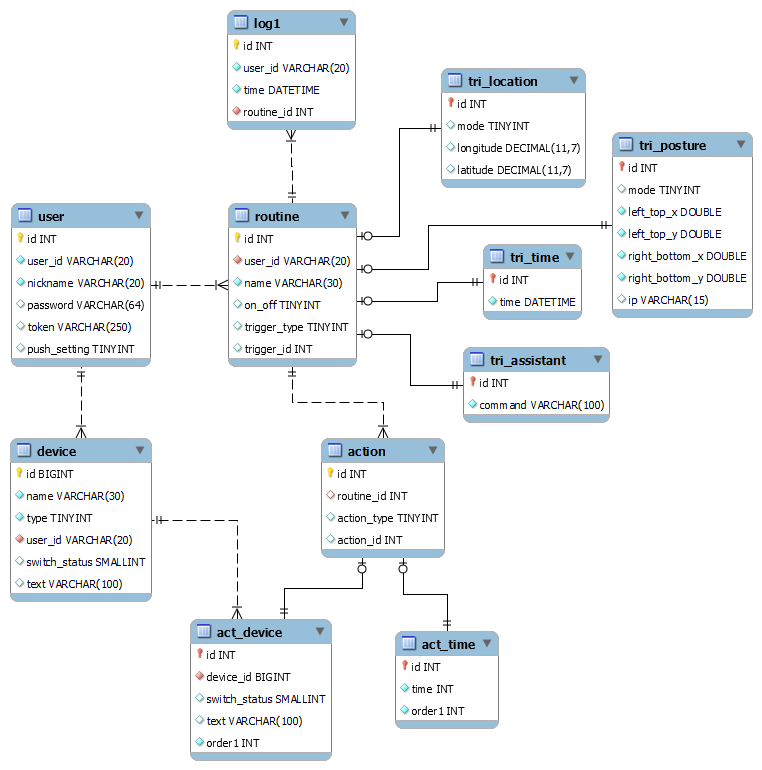
\includegraphics[width=12cm]{imgs/architecture_design_and_implementation/database-erd.png}
                    \caption{Database ERD} 
                    \renewcommand{\thefigure}{\thesubsection.\arabic{figure}}
                \end{center}
            \end{figure*}
          % \addImage{
          %     imgs/architecture_design_and_implementation/database-erd.png
          % }{
          %     Database Diagram
          % }
          This is the database that our architecture is currently using. This database consists of 11 tables. By using the structure of these tables, the data generated by the project can be stored.\\
          \begin{enumerate}
              \item user
                    \begin{itemize}
                        \item Used to store registered user information.
                        \item Primary Key: id (auto-increment, unique identifier in the user table), used for indexing data in the table.
                        \item user\_id: varchar(30), a unique identifier for the user. Used to differentiate between different users in the system.
                        \item nickname: varchar(30), the user's nickname. Displayed on the user interface for personalizing the user experience.
                        \item password: varchar(64), the user's password used for authentication during login. Should be stored encrypted in MD5 format to ensure data security.
                        \item token: varchar(250), the user's token used for authentication and access control, ensuring the security of sensitive operations.
                        \item push\_setting: tinyint, default value 1, push notification settings; 0 indicates disabled, 1 indicates enabled. Controls the status of push notifications in the app.\\
                    \end{itemize}

              \item device
                    \begin{itemize}
                        \item Used to store information about devices connected by users.
                        \item Primary Key: id (auto-increment, unique identifier in the device table), stored in bigint format to accommodate larger device IDs.
                        \item name: varchar(30), the name of the device used for identification and description, allowing users to customize the device name displayed in the app.
                        \item type: tinyint, device type, used for categorizing and distinguishing different types of devices. For example, when it is 1, it represents a sliding light bulb, 2 is a switch light bulb, 3 is a general switch, and so on. Different control components are displayed in the app based on the device type.
                        \item user\_id: varchar(20), linked to the user\_id in the user table, used to identify the owner of the device, ensuring that the device is associated with a specific user.
                        \item switch\_status: smallint, default value 0, represents the on/off status of the device, with values ranging from 0 to 100, indicating the current state of the device.
                        \item text: varchar(100), the device's IP address or command, used for communication and control of the device or for storing other necessary information.\\
                    \end{itemize}

              \item routine
                    \begin{itemize}
                        \item Used to store various routine information saved by users.
                        \item Primary Key: id (auto-increment, unique identifier in the routine table), used for indexing data in the table.
                        \item user\_id: varchar(20), linked to the user\_id in the user table, identifying the owner of the routine, ensuring that the routine is associated with a specific user.
                        \item name: varchar(30), the name of the routine, used to save the user-set routine name.
                        \item on\_off: tinyint, default value 0, the on/off status of the routine, where 0 indicates off and 1 indicates on, controlling the activation status of the routine.
                        \item trigger\_type: tinyint, trigger type, used to indicate which type of trigger will activate this routine. For example, 1 represents location-based triggering, and 2 represents posture recognition triggering.
                        \item trigger\_id: int, linked to the IDs in various trigger tables, used to establish the association between the routine and trigger conditions.\\
                    \end{itemize}

              \item tri\_location
                    \begin{itemize}
                        \item This table is used to store location-based trigger information.
                        \item Primary Key: id (auto-increment, unique identifier in the location trigger table), used for indexing data in the table.
                        \item mode: tinyint, default value 0, mode where 0 represents triggering on entry, and 1 represents triggering on exit. Determines the type of location trigger.
                        \item longitude: decimal(11, 7), longitude representing the coordinates of the location. Used to define the geographic location for location-based triggering.
                        \item latitude: decimal(11, 7), latitude representing the coordinates of the location. Used to define the geographic location for location-based triggering.\\
                    \end{itemize}

              \item tri\_posture
                    \begin{itemize}
                        \item Used to store the screen range to be recognized by the camera.
                        \item Primary Key: id (auto-increment, unique identifier in the posture trigger table), used for indexing data in the table.
                        \item mode: tinyint, default value 0, mode where 0 represents sitting posture triggering, 1 represents standing posture triggering, and 2 represents lying posture triggering. Used to determine the type of posture trigger.
                        \item left\_top\_x: double, the X coordinate of the top-left corner used to define the x-axis of the top-left corner of the posture trigger area. Determines the triggering area for posture recognition.
                        \item left\_top\_y: double, the Y coordinate of the top-left corner used to define the y-axis of the top-left corner of the posture trigger area. Determines the triggering area for posture recognition.
                        \item right\_bottom\_x: double, the X coordinate of the bottom-right corner used to define the x-axis of the bottom-right corner of the posture trigger area. Determines the triggering area for posture recognition.
                        \item right\_bottom\_y: double, the Y coordinate of the bottom-right corner used to define the x-axis of the bottom-right corner of the posture trigger area. Determines the triggering area for posture recognition.
                        \item ip: varchar(15), can be used for the camera's IP address if needed.\\
                    \end{itemize}

              \item tri\_assistant
                    \begin{itemize}
                        \item Used to store characters or sentences that need to be recognized.
                        \item Primary Key: id (auto-increment, unique identifier in the assistant trigger table), used for indexing data in the table.
                        \item command: varchar(100), can be used to store an IP address or command for voice recognition.\\
                    \end{itemize}

              \item tri\_time
                    \begin{itemize}
                        \item Used to store the time required for time triggers.
                        \item Primary Key: id (auto-increment, unique identifier in the time trigger table).
                        \item time: datetime, stores the trigger time, used to specify when operations related to this time should be triggered.\\
                    \end{itemize}

              \item action
                    \begin{itemize}
                        \item Serves as the main table for actions, allowing data related to actions to be retrieved based on their types and IDs.
                        \item Primary Key: id (auto-increment, unique identifier in the action table), used for indexing data in the table.
                        \item routine\_id: int, linked to the ID in the routine table, indicating the routine associated with this action. Establishes the association between actions and routines.
                        \item action\_type: tinyint, action type, where 1 represents device actions and 2 represents time-delayed time actions. Used to determine the type of action.
                        \item action\_id: int, linked to the ID in the corresponding action type table. Using the action type data and action ID, specific information about the action can be retrieved.\\
                    \end{itemize}

              \item act\_device
                    \begin{itemize}
                        \item Used to store the state to which devices should be changed after action triggers.
                        \item Primary Key: id (auto-increment, unique identifier in the device action table), used for indexing data in the table.
                        \item device\_id: bigint, linked to the ID in the device table, indicating the device to be controlled. Establishes the association between actions and devices.
                        \item switch\_status: smallint, default value 0, represents the switch status to be modified by the action, with values ranging from 0 to 100.
                        \item text: varchar(100), used to store the device's IP address or command, specifying the specific operation of the device action.
                        \item order1: int, indicates the order in which the action should be executed. Used to determine the execution order when multiple actions are present.\\
                    \end{itemize}

              \item act\_time
                    \begin{itemize}
                        \item Stores the specific time for delayed triggers.
                        \item Primary Key: id (auto-increment, unique identifier in the time action table), used for indexing data in the table.
                        \item time: int, time in seconds, indicating the time delay for executing the action. Used to specify the triggering time for time actions.
                        \item order1: int, indicates the order in which the action should be executed. Used to determine the execution order when multiple actions are present.\\
                    \end{itemize}

              \item log1
                    \begin{itemize}
                        \item Stores log trigger records.
                        \item Primary Key: id (auto-increment, unique identifier in the log table), used for indexing data in the table.
                        \item user\_id: varchar(20), linked to the user\_id in the user table, indicating the user to whom the log belongs. Ensures that the log is associated with a specific user.
                        \item time: datetime, records the time the log was generated. Used to track the time of events.
                        \item routine\_id: int, linked to the ID in the routine table, indicating the routine associated with the log. Used to indicate which routine triggered this log record.\\
                    \end{itemize}

          \end{enumerate}
    \item Class Component \\
    \item[-] pom.xml: This file is associated with the Maven build management tool commonly used in Java projects. It contains project configuration information and is written in XML format. It is used to define project settings, dependencies, plugins, and other build-related information.\\
    \item[-] src/main/resources/application.properties : This configuration file defines settings for a Spring Boot application, specifying the context path as "/api" and providing connection details for a MySQL database.\\
    \item[-] src/main/java/com.tempomate/controller: This is the folder that contains controllers which handle user input and return the results to the user. \\
    \item[-] ActionController: This class handles API operations related to actions using POST, GET, and DELETE mappings. The "/actDevice\_add" and "/actTime\_add" endpoints use POST requests to respectively add device actions and time delay actions. The "/get\_all\_action/\{userId\}" endpoint retrieves all actions stored in the database using a GET request, where \{userId\} is the user identifier. The "/delete/\{id\}" endpoint deletes the action corresponding to the provided ID from the database using a DELETE request.\\
    \item[-] DeviceController: This class handles various mappings related to devices, including POST, DELETE, GET, and PUT. The "/add" endpoint uses POST to add a device to the database. The "/delete/\{id\}" endpoint, using DELETE, removes the device with the specified ID from the database. The "/get\_all\_device/\{userId\}" endpoint, with GET, returns all devices associated with the given user ID. The "/rename\_device" endpoint, using PUT and receiving a new device name in the request body, updates the device name. Lastly, the "/change\_status" endpoint, through PUT, receives a request to change the device's switch within the range of 0 to 100. \\
    \item[-] LogController: This class handles logging, and the "/user/\{userId\}" endpoint, through a GET mapping, returns a list of all logs for the user corresponding to the user ID in the endpoint. \\
    \item[-] RoutineController: This class handles various mappings related to routines, encompassing POST, DELETE, GET, and PUT methods. The "/add" endpoint is used to create a new routine using a POST request. The "/delete/\{id\}" endpoint, through a DELETE mapping, processes the deletion of the routine associated with the provided ID. The "/get\_all\_routine/\{userId\}" endpoint, utilizing the GET method, returns a list of all routines associated with the specified `\{userId\}` value. The "/rename\_routine" endpoint, receiving a request for a new routine name, updates the routine's name using a PUT request. Finally, the "/change\_status" endpoint, taking the routine's ID and on/off status in the request body, updates the routine's on/off status using a PUT request. \\
    \item[-] TriggerController: This class uses POST mappings to add triggers and GET mappings to retrieve them. The endpoints "/loc\_add," "/pos\_add," "/assi\_add," and "/time\_add" are used to respectively add location triggers, posture triggers, assistant triggers, and time triggers through POST requests. The "/get" endpoint receives triggerType and triggerId in the request and returns the corresponding trigger using a POST mapping. Additionally, conditional statements are used to fetch different triggers based on the trigger type of the routine. For each trigger type, it retrieves the appropriate trigger (TriLocation, TriPosture, TriAssistant, TriTime) from the database. \\
    \item[-] UserController: This class handles user-related information using POST and PUT mappings. The "/signup" endpoint deals with user registration using a POST request. The "/login" endpoint is a POST API that receives the user's ID and password in the request for performing login. The "/rename-nickname" endpoint updates the user's nickname by receiving a new nickname through a PUT request. The "/push\_setting" endpoint manages the user's push notification status using a PUT request.\\
    \item[-] src/main/java/com.tempomate/exception/ \par GlobalExceptionHandler: This code defines a global exception handler in a Spring Boot application.\\
    \item[-] src/main/java/com.tempomate/mapper : This is the folder that is employed to define and execute SQL queries for interacting with a database. \\
    \item[-] ActionMapper: This interface interacts with the database to provide functionality related to actions. The `addAction`, `addActDevice`, and `addActTime` methods are responsible for adding action, device action, and time delay action, respectively, to the database. The `getActDevice` and `getActTime` methods retrieve device actions and time delay actions associated with a user and routine. Lastly, the `deleteAction` method removes all action data from the database. \\
    \item[-] DeviceMapper: This interface handles database operations for the `Device` entity. It includes methods to add a new device, retrieve all devices associated with a specific user, delete a device based on its ID, rename a device, and update the switch status of a device. \\
    \item[-] LogMapper : This interface handles database retrieval operations related to the `Log` entity. The `get\_all\_log` method retrieves all logs associated with a specific user ID from the database.\\
    \item[-] RoutineMapper: This interface manages database operations related to the `Routine` entity. It includes methods for adding a new routine, deleting a routine based on a specific ID, renaming a routine, and updating the active/inactive status of a routine. \\
    \item[-] TriggerMapper: This interface is responsible for handling database operations related to triggers in the context of routines. This includes methods for adding triggers of different types (location, posture, assistant, and time) and retrieving specific trigger information based on the trigger ID associated with a routine. \\
    \item[-] UserMapper: This interface handles database operations related to user management. It includes methods for retrieving a list of users (primarily used for testing purposes), inserting a new user, performing user login authentication, changing a user's nickname, and updating the push notification settings for a user. \\
    \item[-] src/main/java/com.tempomate/pojo/entity : This is the folder that contains all entity files. \\
    \item[-] ActDevice: This code defines a ‘ActDevice' entity representing device action information, utilizing Lombok annotations for concise code. The entity includes fields for an ID (‘id’), routine ID (‘routineId’), device ID (‘deviceId’), switch status (‘switchStatus’), text (‘text’), and action order ('order1'), allowing for a simplified representation of these attributes.\\
    \item[-] Action: This code defines a ‘Action' entity representing action information, utilizing Lombok annotations for concise code. The entity includes fields for an ID (‘id’), routine ID (‘routineId’), action type (‘actionType’), and action ID (‘actionId’), allowing for a simplified representation of these attributes. \\
    \item[-] ActTime: This code defines a ‘ActTime' entity representing time delay action information, utilizing Lombok annotations for concise code. The entity includes fields for an ID (‘id’), routine ID (‘routineId’), timestamp (‘time’), and action order ('order1'), allowing for a simplified representation of these attributes.\\
    \item[-] TriAssistant: This code defines a ‘TriAssistant' entity representing assistant trigger information, utilizing Lombok annotations for concise code. The entity includes fields for an ID (‘id’), and command (‘command’), allowing for a simplified representation of these attributes.\\
    \item[-] TriLocation: This code defines a ‘TriLocation' entity representing location trigger information, utilizing Lombok annotations for concise code. The entity includes fields for an ID (‘id’), user action (‘mode’), longitude (‘longitude’), and latitude (‘latitude’), allowing for a simplified representation of these attributes.\\
    \item[-] TriPosture: This code defines a ‘TriPosture' entity representing posture trigger information, utilizing Lombok annotations for concise code. The entity includes fields for an ID (‘id’), user action (‘mode’), left top-X (‘leftTopX’), left top-Y (‘leftTopY’), right bottom-X ('rightBottomX'), right bottom-Y ('rightBottomY') and IP address (‘ip’), allowing for a simplified representation of these attributes. \\
    \item[-] TriTime: This code defines a ‘TriTime' entity representing time trigger information, utilizing Lombok annotations for concise code. The entity includes fields for an ID (‘id’), and timestamp (‘time’), allowing for a simplified representation of these attributes.\\
    \item[-] Device: This code defines a ‘Device' entity representing device information, utilizing Lombok annotations for concise code. The entity includes fields for an ID (‘id’), name (‘name’), device type (‘type’), user ID (‘userId’), switch status (‘switchStatus’), and text (‘text’), allowing for a simplified representation of these attributes.\\
    \item[-] Log: This code defines a ‘Log' entity representing log information, utilizing Lombok annotations for concise code. The entity includes fields for an ID (‘id’), user ID (‘userId’), timestamp (‘time’), and routine ID (‘routineId’), allowing for a simplified representation of these attributes. \\
    \item[-] Routine: This code defines a ‘Routine' entity representing routine information, utilizing Lombok annotations for concise code. The entity includes fields for an ID (‘id’), user ID (‘userId’), name (‘name’), switch status (‘onOff’), trigger type (‘’triggerType’) and trigger ID (‘triggerId’), allowing for a simplified representation of these attributes.\\
    \item[-] User: This code defines a ‘User' entity representing user information, utilizing Lombok annotations for concise code. The entity includes fields for an ID (‘id’), user ID (‘userId’), nickname (‘nickname’), password (‘password’), token (‘token’), and push notification setting (‘pushSetting’), allowing for a simplified representation of these attributes.\\
    \item[-] src/main/java/com.tempomate/pojo/result: This class provides a standardized method for encapsulating and conveying response results in a unified format across various parts of the application.\\
    \item[-] src/main/java/com.tempomate/service: This folder is responsible for handling business logic, coordinating data access, and performing various operations.\\
    \item[-] UserServiceImpl: This code defines the `UserServiceImpl` class, which implements the `UserService` interface. The class encapsulates the logic for user-related services, utilizing the `UserMapper` to interact with the database. Each method takes a `User` object as a parameter, performs the corresponding functionality, and returns the result.\\
    \item[-] UserService: This code defines the `UserService` interface, specifying methods for user-related operations such as user registration (`userSignup`), user login (`login`), changing a user's nickname (`change\_nickname`), and managing user push notification settings (`push\_setting`).\\
\end{enumerate}
\item APIs
\begin{enumerate}
    \item /action
    \item[-] /actDevice\_add: This API is designed to add a new device action (`ActDevice`) and create a corresponding action (`Action`). Users can submit a POST request with the information for the new device action in the request body. The system utilizes the "addActDevice" method to add the new device action and generates a related action using the "addAction" method. The action includes the routine ID, action type, and the ID of the added action. Upon successful completion, the system logs the ID of the added device action and returns that ID as part of the success response.\\
    \item[-] /actTime\_add: This API is designed to add a new time delay action (`ActTime`) and create a corresponding action (`Action`). Users can submit a POST request with the information for the new time delay action in the request body. The system utilizes the "addActTime" method to add the new time delay action and generates a related action using the "addAction" method. The action includes the routine ID, action type, and the ID of the added action. Upon successful completion, the system logs the ID of the added time delay action and returns that ID as part of the success response.\\
    \item[-] /get\_all\_action/\{userId\}: This API provides functionality to retrieve all actions associated with a specific user. Users can send a GET request with the user ID and routine ID in the request body. The system uses the "getActDevice" and "getActTime" methods to fetch all device actions and time delay actions for the specified user and routine. The retrieved results are logged, and a success response containing the action device and action time lists is returned to the user.\\
    \item[-] /delete/\{id\}: This API provides functionality to delete the action. Users can send a DELETE request with action ID and action type in the request body. The system uses the "deleteAction" method to remove the specified action from the database, checks the number of affected rows, and then deletes action information from actDevice table or actTime table based on the action type. Upon successful deletion, the API responds with a success message, and if no rows are deleted, it returns an error response with the message "no match."\\
    \item /device
    \item[-] /add: This API allows users to add a new device by sending a POST request with device information in the request body. The system utilizes the "add\_device" method in the DeviceMapper to insert the device details into the database. Upon successful addition, the system logs the user ID performing the operation, logs the ID of the newly added device, and returns a success response containing the device ID.\\
    \item[-] /delete/\{id\}: This API provides functionality to delete a specific device. Users can send a DELETE request with the ID of the device they wish to delete specified as a path variable. The system uses the "delete\_device" method to remove the corresponding device from the database and returns the number of affected rows. Based on the result, the API responds with a success message if the operation is successful or an error message if it fails.\\
    \item[-] /get\_all\_device/\{userId\}: This API retrieves all devices associated with a specific user. Users can send a GET request with their user ID specified as a path variable. The system uses the "get\_all\_device" method to fetch the list of devices from the database based on the provided user ID. The API responds with a success message containing the list of devices associated with the specified user.\\
    \item[-] /rename\_device: This API allows users to rename a device by sending a PUT request with the device ID and the updated device name in the request body. The system utilizes the "rename\_device" method, which executes an SQL UPDATE statement to change the name of the specified device in the database. Upon successful completion, the API responds with a success message, including the updated device name.\\
    \item[-] /change\_status: This API enables users to modify the switch status of a device by sending a PUT request with the device Id and the updated device status in the request body. The system validates that the provided switch status is within the range of 0 to 100. If the validation is successful, the system uses the "change\_status" method to update the device's switch status in the database. Upon successful completion, the API responds with a success message containing the updated switch status. If the provided switch status is outside the valid range, an error response is returned, and an error message is logged.\\

    \item /log
    \item[-] /user/\{userId\}: This API retrieves all logs associated with a specific user by sending a GET request with the user ID specified as a path variable. The system uses the "get\_all\_log" method, which executes an SQL SELECT statement to fetch log entries from the database based on the provided user ID. The API responds with a success message containing the list of log entries associated with the specified user.\\

    \item /routine
    \item[-] /add: This API provides functionality to add a new routine. Users can send a POST request with routine information in the request body. The system uses the "add\_routine" method to insert the new routine details into the database. Upon successful addition, the system logs the user ID performing the operation, logs the ID of the newly added routine, and returns a success response containing the routine ID.\\
    \item[-] /delete/\{id\}: This API allows users to delete a specific routine by sending a DELETE request with the routine ID specified as a path variable. The system utilizes the "delete\_routine" method to remove the corresponding routine from the database and returns the number of affected rows. Based on the result, the API responds with a success message if the operation is successful or an error message if it fails.\\
    \item[-] /get\_all\_routine/\{userId\}: This API retrieves all routines associated with a specific user by sending a GET request with the user ID specified as a path variable. The system uses the "get\_all\_routine" method to fetch the list of routines from the database based on the provided user ID. The API responds with a success message containing the list of routines associated with the specified user.\\
    \item[-] /rename\_routine: This API allows users to rename a routine by sending a PUT request with the routine ID and the updated routine name in the request body. The system utilizes the "rename\_routine" method, which executes an SQL UPDATE statement to change the name of the specified routine in the database. Upon successful completion, the API responds with a success message containing the updated routine name.\\
    \item[-] /change\_status: This API allows users to toggle the active/inactive status of a routine by sending a PUT request with the routine ID and the updated routine activation setting (0 or 1) in the request body. The system utilizes the "change\_status" method, which executes an SQL UPDATE statement to toggle the on/off status of the specified routine in the database. Upon successful completion, the API responds with a success message containing the toggled on/off status. Otherwise, an error response with the message "fail to toggle push setting" is returned.\\

    \item /trigger
    \item[-] /loc\_add: This API enables users to add a new location trigger (TriLocation) by sending a POST request with the location trigger information in the request body. The system uses the "triLocationAdd" method to insert the new location trigger details into the database. Upon successful addition, the system logs the ID of the newly added location trigger and returns a success response containing that ID.\\
    \item[-] /pos\_add: This API enables users to add a new posture trigger (TriPosture) by sending a POST request with the posture trigger information in the request body. The system uses the "triPostureAdd" method to insert the new posture trigger details into the database. Upon successful addition, the system logs the ID of the newly added posture trigger and returns a success response containing that ID.\\
    \item[-] /assi\_add: This API enables users to add a new assistant trigger (TriAssistant) by sending a POST request with the assistant trigger information in the request body. The system uses the "triAssistantAdd" method to insert the new assistant trigger details into the database. Upon successful addition, the system logs the ID of the newly added assistant trigger and returns a success response containing that ID.\\
    \item[-] /time\_add: This API enables users to add a new time trigger (TriTime) by sending a POST request with the time trigger information in the request body. The system uses the "triTimeAdd" method to insert the new time trigger details into the database. Upon successful addition, the system logs the ID of the newly added time trigger and returns a success response containing that ID.\\
    \item[-] /get: This API provides functionality to retrieve trigger information associated with a routine. Users can send a POST request with the trigger ID and the trigger type of routine table in the request body. Depending on the trigger type and trigger ID in the routine, the system uses specific methods to fetch corresponding trigger information from the database. After retrieving information for each trigger type, it returns a success response containing the relevant information, or an error response with the message "no match" if no information is found.\\

    \item /user
    \item[-] /signup: This API allows new users to sign up by sending a POST request with user information in the request body. The provided information is then inserted into the user table using the "insertUser" method in the UserMapper.\\
    \item[-] /login: This API enables users to log in by sending a POST request with their user credentials in the request body. The system logs the login attempt, including the user ID and password. The login credentials are then verified against the user table using the "login" method in the UserMapper. If the credentials are valid (resulting in a count of 1), the API returns a success response; otherwise, it returns an error response.\\
    \item[-] /rename-nickname: This API allows users to change their nickname. Users can submit a PUT request with the new nickname in the request body. The system updates the user's ID with the specified nickname, and upon successful completion, it returns the updated nickname as part of the response. The system logs the attempt to change the nickname, including the user's ID.\\
    \item[-] /push\_setting: This API is designed for toggling the push notification setting of a user. Users can send a PUT request with the user ID and the current push setting status in the request body. The system logs the attempt to toggle the push notification setting, updates the user's push setting (switching between 0 and 1), and returns the updated push setting as part of the response in case of success. If the operation is successful (resulting in a count of 1), the API responds with the updated push setting; otherwise, it returns an error message indicating a failure to toggle the push setting. The actual push setting update is implemented in the "push\_setting" method, which executes an SQL UPDATE statement on the user table.\\
\end{enumerate}

                \newpage
              \item Computer vision\\
                                    \begin{enumerate}
                        \item Purpose\\
                              The computer vision part of TempoMate has a simple job to do.
                              It receives video information from a connected camera, and then sends it to the client via the backend so that when an event occurs that corresponds to a posture trigger you've set up, the client that has that routine will execute it.\\\\

                        \item Funtionality\\
                              \begin{enumerate}
                                  \item Camera connection:\\
                                        Since Matter doesn't support cameras, we need to get footage directly from the user's own camera in some other way. We get the camera footage from the backend via the RTMP protocol.\\

                                  \item pose recognition:\\
                                        After fetching the camera footage in real-time, we analyze the camera's screen at 30 frames per second to find out if a person is present and, if so, in what position. The data found is represented by a dot on the top left of the box representing the person, a dot on the bottom right, and finally a pose.\\

                                  \item Normalize the data:\\
                                        Since different cameras have different resolutions, we represent the coordinates as floating-point points corresponding to 0-1. Also, since people can move, we cluster data in similar locations. Since there is a possibility of model malfunction, we filter out the 30 frames per second that we recognize more than a certain number of times.\\

                                  \item Enable triggers:\\
                                        Using the normalized data and the trigger data received through the backend, we analyze if there are any triggers that can be activated. If a person's pose remains in one position, it is handled appropriately to prevent multiple triggers.\\\\
                              \end{enumerate}
                        \item Location of source code \\
                              : www.github.com/se-tmp/backend \\\\

                        \item Class Component\\
                              \begin{enumerate}
                                  \item processing\\
                                        The contents of this folder are actually about the services that work for the entire project.\\

                                  \item model.pt\\
                                        This file is an integral part of the project, allowing us to determine if a person is in a particular frame of a video, and if so, what pose they are in.\\

                                  \item ThreadedCamera.py\\
                                        This class allows you to receive camera video from the backend via the RTMP protocol. It determines the frames in the video, fetches the frame information back at the time corresponding to each frame, and passes it to another class.\\

                                  \item Processor.py\\
                                        This class normalizes and clusters the data we get from the model. It uses this data to find out if any of the triggers fetched from the backend should be activated. \\

                                  \item main.py\\
                                        This file initiates the camera connection, receives frames from the ThreadedCamera, analyzes the frames through the model, and passes the results to the Processor class.\\
                              \end{enumerate}

                        \item training/train.ipynb\\
                              This file is where we actually train the model using the dataset.\\
                    \end{enumerate}

          \end{enumerate}
\end{enumerate}

\clearpage
\bibliographystyle{IEEEtran}
\bibliography{references}

% \section{\Large{Architecture Design \& Implementation}}
% \begin{enumerate}[label=\arabic*]
%     \item {\large{Overall Architecture}}\\
%     \begin{figure}[H]
%         \centering
%         \includegraphics[scale=0.2]{images/overallarchitecture.eps}
%     \end{figure}
%     This is the Our service consists of five modules. Each is front-end, back-end, database, machine learning, and IoT such as AI speaker and smart mirror. Among them, front-end and IoT are modules that directly communicate with users. \\
%     The first module is the front-end. We used JavaScript language and React Native, a cross-platform framework that supports both Android and IOS as a mobile application framework. So, all household members can use our application regardless of their smart phone model. Through the application, the user can belong to the household and check the appropriate carbon emission reduction behavior. In addition, users can check the amount of carbon they can reduce when they practice carbon emission reducing efforts in each behavioral area and the amount of carbon emission they are currently emitting in each behavioral area.\\
%     The second is the back-end. We used the Django framework based on the Python language as the web application server framework. In addition, uWSGI was used as wsgi middleware that connects web server and web application server. And nginx was used as the web server. The backend largely communicates with three devices: application, AI speaker, IoT such as smart mirror. So, the server is implemented in the form of providing REST API. When the AI speaker notifies the server that the user has started/ended the carbon emission reduction behavior, the server stores it to the database. Also, the server responds when the application requests the user’s information.\\
%     Third, it is a database.  We used mysql as a database. Mysql is an RDBMS, we store user information, user behavior practice records, information related to user behavior practice, and previous dataset statistics.\\
%     The fourth is machine learning. We predict the most appropriate shower shortcut time through the user’s first shower time. Reducing the shower time by 1 minute has a problem of presenting an absolute value without considering the shower time of the user. Therefore, there is a problem in that users try to reduce 1minute even though they can reduce more time without experiencing inconvenience. Therefore, we present an AI model that presents an appropriate reduction for the user’s shower time.\\
%     Lastly, it is IoT. We used AI speakers to interact with users by voice when practicing carbon emission reduction behavior, making it easier to use the service in more diverse situations. Voice interaction services are developed using existing development tools. In the case of smart mirrors, raspberry pie was used.\\
    
%     \item {\large{Directory Organization}}\\
%     \begin{enumerate}[label=\alph*]
%         \item front end
% \begin{flushleft}
%         \tablefirsthead{\toprule Directory & File name & etc \\}
%         \tablehead{\toprule Directory & File name & etc\\}
%         \tabletail{\midrule}
%         \tablelasttail{\bottomrule}
%         \begin{supertabular}{p{0.5\linewidth} | p{0.3\linewidth} p{0.05\linewidth}}
%         \midrule
%         /front-end & \makecell[l]{.eslintrc.js\\.gitignore\\.prettierrc.js\\.watchmanconfig\\app.json\\babel.config.js\\index.jsx\\package.json} \\
%         \midrule
        
%         /front-end/apps	& App.jsx \\
%         \midrule
        
%         /front-end/apps/assets & \makecell[l]{environmenttw.png\\globe.png\\globew.png\\logo.png\\logo2.png}\\
%         \midrule
        
%         \makecell[l]{//front-end/apps\\/navigator} & \makecell[l]{mainNavigator.jsx\\signInNavigator.jsx\\bottomTabNavigator.jsx}\\
%         \midrule
        
%         \makecell[l]{/front-end/apps\\/components/api} & axios.jsx\\
%         \midrule

%         \makecell[l]{/front-end/apps\\/components/common} & wrapper.jsx\\
%         \midrule
        
%         \makecell[l]{/front-end/apps\\/components/context} & tokenContext.jsx\\
%         \midrule
        
%         \makecell[l]{/front-end/apps\\/components/navigator} & \makecell[l]{bottomTabNavigator.jsx\\ GraphDetailsNavigator.jsx\\graphNavigator.jsx\\loginNavigator.jsx\\mainNavigator.jsx}\\
%         \midrule

%         \makecell[l]{/front-end/apps\\/components/screens\\/main} & main.jsx\\
%         \midrule
        
%         \makecell[l]{/front-end/apps\\/components/screens\\/signUp} & signUp.jsx\\
%         \midrule
        
%         \makecell[l]{/front-end/apps\\/components/screens\\/signIn} & signIn.jsx\\
%         \midrule
        
%         \makecell[l]{/front-end/apps\\/components/screens\\/home} & home.jsx\\
%         \midrule
        
%         \makecell[l]{/front-end/apps\\/components/screens\\/recommended} & recommended.jsx\\
%         \midrule
        
%         \makecell[l]{/front-end/apps\\/components/screens\\/records} & records.jsx\\
%         \midrule
        
%         \makecell[l]{/front-end/apps\\/components/screens\\/profile} & \makecell[l]{profile.jsx\\ myPageList.jsx}\\
%         \end{supertabular}
% \end{flushleft}
        
%         \item back end
%         \begin{flushleft}
%         \tablefirsthead{\toprule Directory & File name & etc \\ \midrule}
%         \tablehead{\toprule Directory & File name & etc\\ \midrule}
%         \tabletail{\midrule }
%         \tablelasttail{\bottomrule}
%         \begin{supertabular}{p{0.5\linewidth} | p{0.3\linewidth} p{0.05\linewidth}}
%         /server & \makecell[l]{.gitignore\\ manage.py}\\
%         \midrule
%         /server/app & \makecell[l]{\_\_init\_\_.py\\admin.py\\apps.py\\models.py\\serializer.py\\tests.py\\views.py}\\
%         \midrule
%         /server/config & \makecell[l]{\_\_init\_\_.py\\asgi.py\\settings.py\\urls.py\\wsgi.py}\\
%         \midrule
%         /server/app/migration & \makecell[l]{0001\_initial.py\\002\_auto\_2021\\        1126\_1010.py\\ \_\_init\_\_.py}\\
%         \midrule
%         /server/auth/migration & \makecell[l]{0001\_initial.py\\ \_\_init\_\_.py}\\
%         \end{supertabular}
% \end{flushleft}
        
%     \end{enumerate}
    
%     \item {\large{Module 1 : front end}}
%     \begin{enumerate}[label=\alph*]
%         \item Purpose\\
%         It is used to provide users with records of behavioral practices. It is also used to guide how to practice behavior. And it is to receive user information and manage household members.
%         \item Functionality\\
%         First of all, it provides a function of managing user information and household members, checking emissions for each behavior of the current user, and checking the amount of carbon that can be reduced. It also provides a function of checking average emissions in the group under the same conditions and checking carbon emission records due to daily and monthly behavior practice. Finally, it provides the function of checking how to practice carbon emission reduction behavior.
%         \item Location of Source Code\\
%         /front-end
%         \item Class Component
%         \begin{enumerate}
%             \item Main Page\\
%             It is the first component to be output when running the app. It is implemented as a functional component, and there is a style sheet representing css. The buttons in the component are imported from the common folder. The logo is imported from the assets folder.
%             \item Sign In Page\\
%             There is an inputText that receives an ID and password. The ID and password are managed through global variables within the file. When clicking the login button, put the ID and password in the request body and send a post request to the server.At this time, communication with the server uses the axios library and is processed asynchronously. React hooks are used to process asynchronous actions in functional components.
%             \item Sign Up Page\\
%             Because we need to receive a lot of information from the user over multiple pages when signing up, we manage multiple components within one file. This makes it easy to manage variables that have received user information without using additional status management libraries.
%             \item Home Page\\
%             This is the default routing page of the bottom tab bar. Page navigation was implemented through the React Navigation Library. The circular graph on the main page also used the graph library. The amount of emissions output in the screen is received through communication with the server when the page is first rendered.
%             \item Records Page\\
%             This page shows the daily and monthly records. Every time you click on that button, data is retrieved through communication with the server.
%             \item Recommended Action Page\\
%             When the user clicks on the list showing each behavior, it shows detailed information through modal. If you press the OK button, the modal window turns off. In the details, my emissions for the behavior, the average emissions of people in the same group as me, and the amount of carbon that can be reduced are output.
%             \item My Page\\
%             You can manage your information and household members on my page. At this time, only the householder is authorized to manage the household members. Permission status is processed by the server. The list of household members is implemented through the React flat list. In addition, the information received when modifying the information is managed as a global variable, and is delivered to the server when the modification button is clicked.
%         \end{enumerate}
%         \item Where it's taken from\\
%         Data is directly input by the user, or previous data is retrieved from db.
%         \item How/Why we used the module\\
%         React Native was used because it is a cross-platform framework that supports both Android and IOS. Since it mainly shows the user's record, it is used in the form of outputting the data when the user's data is retrieved from the server.
%     \end{enumerate}
    
%     \item {\large{Module 2 : back end}}
%     \begin{enumerate}[label=\alph*]
%         \item Purpose\\
%         Our service helps with various behaviors at home. Therefore, it should be linked with not only applications but also smart mirrors and AI speakers. For this reason, a server that manages many devices in an integrated manner was needed.
%         \item Functionality\\
%         It mainly provides REST APIs that respond to requests when sent from clients. When the client requests db's data, it inquires db and delivers the information to the client. Or it is in charge of communication between connected devices.
%         \item Location of Source Code\\
%         / server
%         \item Class Component
%         \begin{enumerate}
%             \item app/views.py\\
%             It is a part that is responsible for the core functions of our service, such as responding to user information requests and recording behavioral practices. This part is responsible for core business logic, and the view corresponding to the controller among the MVC patterns is implemented as a class-based view (CBV). Each function has each endpoint.
%             \item app/models.py\\
%             It is a file responsible for automatically connecting data from objects and databases. This makes it easier to access values in the database from Django. In this file, all tables in the database appear as objects.
%             \item app/serializer.py\\
%             This file serves to make the response value in the appropriate form to communicate with. All of the values modified in view are not in a bonded form to communicate with the client. Therefore, we need to make the value in an appropriate form. The client and server communicate in the form of JSON, so the serializer classes change the value to JSON form in this file.
%             \item config/urls.py\\
%             It is a file that manages endpoints for communication. It also connects endpoints and views. Endpoints for all requests are set here.
%         \end{enumerate}
%         \item Where it's taken from\\
%         In terms of data, data comes from applications, databases and various IoT such as AI speakers and smart mirrors.
%         \item How/Why we used the module\\
%         Django was used because it is a web application framework based on Python, the most common language. In addition, nginx and uWSGI were used to provide more stable services. The WAS was built in Django, and the web server was built in nginx. And they were connected by uWSGI.
%     \end{enumerate}
    
%     \item {\large{Module 3 : database}}
%     \begin{enumerate}[label=\alph*]
%         \item Purpose\\
%         We constructed a database to systematically store a lot of data generated when users practice carbon emission reduction behavior.  This is also because data with a fixed format must be stored steadily. So we chose MySQL, which is RDBMS. It is also for better AI modeling through data accumulation.
%         \item Functionality\\
%         It provides systematic data management through tables. In addition, relationships can be expressed through foreign keys between tables, enabling more efficient space management. In addition, we can easily manipulate a lot of data through query statements.
%         \item Location of Source Code
%         \begin{enumerate}
%             \item /server/app/models.py - we can check the DB in the form of ORM in the server directory. 
%             \item on aws rds
%         \end{enumerate}
%         \item Class Component
%         \begin{enumerate}
%             \item auth\_user\\
%             A table that stores user information. It is a user table provided by Django and can be easily expanded.
%             \item personalShowerData\\
%             A table that stores unchanged values among the user's shower data. It reduces the occurrence of duplicate values by distinguishing them from the shower log table.
%             \item showerLog\\
%             This is a table that stores the user's shower records. It regularly stores data every time a user takes a shower.
%             \item showerDataSet\\
%             This is the data based on the age group of the dataset. This is a table that we refer to when we need information about the same age as the user.
%         \end{enumerate}
%         \item Where it's taken from\\
%         It stores data input from the user. Or save behavioral records when the user practices behavior.
%         \item How/Why we used the module\\
%         First, we used user tables provided by 'Django'. Therefore, there were tables related to user information, and we expanded tables containing user behavior practice information from those tables. a table was created to store the user's behavioral practice records and a table to store invariant values such as the user's target shower time. And a table was created to store statistical content for datasets for ai learning.
%         \begin{figure}[H]
%             \centering
%             \includegraphics[scale=0.14]{images/database.eps}
%         \end{figure}
%     \end{enumerate}
    
%     \item {\large{Module 4 : machine learning}}\\
%     \begin{enumerate}[label=\alph*]
%         \item Purpose\\
%         Our service provides users the group’s carbon emission and the user’s predicted carbon reduction through the application. It invokes users to do the recommended action and set the target for them. Also users can comprehend the validity of the action and the number. In the process, machine learning is essential. \\
%         \item Functionality\\
%         Machine learning enables predicting new user’s carbon emission reduction. As the new application user downloads and signs in, data such as age and gender is sent to the database and his/hers reduction is predicted through the machine learning model we prepared.\\
%         \item Location of Source Code\\
%         ESG\_Home.ipynb
%         \item Class Component\\
%         \begin{enumerate}
%             \item train\_test\_split\\
%             It splits arrays or matrices into random train and test subsets, considering the parameters such as test\_size, train\_size and stratify.
%             \item StandardScaler\\
%             It standardizes features by removing the mean and scaling to unit variance. Standardization of a dataset is a common requirement for many machine learning estimators.
%             \item sklearn.metrics\\
%             It implements functions assessing prediction error for specific purposes. We used r2\_score, mean\_absolute\_error and mean\_squared\_error to evaluate and compare the models.
%             \item LinearRegression\\
%             Linear regression makes predictions by creating a linear function of training data.
%             \[ŷ = w[0] × x[0] + w[1] × x[1] + … + w[p] × x[p] + b\]
%             x[0] to x[p] is the feature and weight w and y-intercept b are parameters learned by the model
%             \item SGDRegressor\\
%             \begin{figure}[H]
%                 \centering
%                 \includegraphics[scale=0.1]{images/AI/sgd_pic.eps}
%             \end{figure}
%              Stochastic Gradient Descent (SGD) is a stochastic gradient descent method that randomly selects a sample from each step and calculates the gradient of the sample.\\
%              It has the advantage of being able to be applied to the large training dataset because it is repeatedly processed with small data and requires only memory for one sample.
%             \item LogisticRegression\\
%             Logistic regression is a supervised learning algorithm that predicts a probability that data falls into a category from 0 to 1 and predicts a category according to that probability. \\
%             Odds is the probability divided by the probability that an event has not occurred. In logistic regression, several features are multiplied by coefficients and intercepts are added to obtain and analyze the final value log-odds.\\
%             The logistic function, also called the sigmoid function, is a function that receives the log-odds obtained above as an input value and outputs a result value between 0 and 1. \\
%             We consider loss to ensure that logistic regression predicts the probability properly, i.e., whether the coefficients and intercepts obtained are appropriate. \\
%             Logistic regression can be seen as having high accuracy when this log loss value is minimized.
%             \item RandomForestRegressor\\
%             \begin{figure}[H]
%                 \includegraphics[scale=0.2]{images/AI/randforest_pic.eps}
%             \end{figure}
%             Random forest is a model that collects regression results from multiple decision trees configured through training and concludes.\\
%             Ensemble learning is a method of using multiple learning algorithms for overfitting prevention and high performance. Random forests initially generate trees through bagging. Bagging is the process of creating a decision tree by selecting some rows of training data, allowing overlapping of rows. Diversity is given to the decision tree by limiting the number of features to be used during this process, usually by the square root of the total number of attributes.
%             \item ExtraTreeRegressor\\
%             Extra trees, also called Extremely randomized trees, are even more random than random forests. Random selection of the number of data samples and feature selection increases prediction accuracy and prevents overfitting.
%             \item GradientBoostingRegressor\\
%             \begin{figure}[H]
%                 \centering
%                 \includegraphics[scale=0.3]{images/AI/gbr_pic.eps}
%             \end{figure}
%             Random forest is a model that collects regression results from multiple decision trees configured through training and concludes.\\
%             The main parameter of gradient boosting is the learning rate, a hyper-parameter that determines how strongly the error in the previous tree will be corrected. Increasing the learning rate creates a complex model because it strengthens correction. Also increasing the n\_estimator value adds more trees to the ensemble, complicating the model and fitting the train data more accurately. To prevent overfitting, you can reduce the depth of the tree or reduce the learning rate.
%             \item AdaBoostRegressor\\
%             AdaBoost is a model that adds weight to the results of other learning algorithms (weak learners). It is also used in combination with many other learning algorithms.\\
%             It is adaptive in that the weak learner can correct the results of incorrect analysis in the previous model. This makes them vulnerable to noise and outliers, but less vulnerable to overfitting than other learning algorithms.
%             \item XGBRegressor\\
%             \begin{figure}[H]
%                 \centering
%                 \includegraphics[scale=0.1]{images/AI/xgb_pic.eps}
%             \end{figure}
%             The Extreme Gradient Boosting model is a model that learns gradient boosting models in parallel.\\
%             Standard gradient boosting models do not have overfitting regulatory features, but XGBoost models are robust with its own overfitting regulatory features.
%             \item LGBMRegressor\\
%             Light GBM is a gradient boosting framework and is a tree-based learning algorithm. Unlike models that scale trees horizontally, LBGM grows trees vertically.\\
%             Even when dealing with large-sized data, memory usage is low, results are fast, and the results are focused on accuracy. LGBM is vulnerable to overfitting and is not used well in small datasets. Our data is a large dataset with 49.027 rows and thus we chose this model. The analysis showed a very high accuracy score, 99.99990470818714\%.
%             \item HistGradientBoostingRegressor\\
%             A histogram-based gradient boosting tree model, suitable for large datasets with more than 10,000 rows. It handles missing values on its own and determines whether the missing values should go to the left or right child during the training process. If missing values that were not in the training process appear during prediction, they are mapped to the child with the most samples.
%             \item permutation\_importance\\
%             It is a model inspection technique that can be used for any fitted estimator when the data is tabular. It is defined to be the decrease in a model score when a single feature is randomly shuffled. By breaking down the relationship between the feature and the target, the model score is indicative of how much the model depends on the feature.\\
%         \end{enumerate}
%         \item Where it's taken from\\
%         Based on the data we provide, models learned to predict the target, which here is reduction. And as the new user signs in, it receives the user’s data from our database and analyzes the reduction of the user.\\
%         \item How/Why we used the module
%         \begin{enumerate}
%             \item pandas\\
%             It’s a software library written for the Python programming language for data manipulation and analysis. In particular, it offers data structures and operations for manipulating numerical tables and time series.
%             \item io\\
%             The io module provides Python’s main facilities for dealing with various types of I/O. It enables reading files and printing outputs.
%             \item numpy\\
%             It is a library for the Python programming language, enabling large, multidimensional arrays and matrices, along with a large collection of high-level mathematical functions to operate on these arrays.
%             \item seaborn\\
%             It is a Python data visualization library based on matplotlib. It provides a high-level interface for drawing attractive and informative statistical graphics.
%             \item matplotlib.pyplot\\
%             It is a collection of functions that make matplotlib work like MATLAB. Each pyplot function makes some changes to a figure, such as creating a figure, creating a plotting area in a figure, plotting some lines in a plotting area and decorating the plot with labels.\\
%         \end{enumerate}
%     \end{enumerate}
    
%     \item {\large{Module 5 : AI speaker \& smart mirror}}
%     \begin{enumerate}[label=\alph*]
%         \item Purpose\\
%         There are many situations in the home where interaction through graphics is difficult, such as bathrooms. We provide voice-based interaction through AI speakers to make the service easier to use in these various situations. In addition, smart mirrors can induce more intuitive behavior to users.\\
%         \item Functionality\\
%         It helps to practice the action of reducing carbon emissions. For example, when the user informs the AI speaker of the start of the shower when taking a shower, the user's proper shower time appears as a timer on the smart mirror.\\
%         \item Location of Source Code
%         \begin{enumerate}
%             \item /smartMirror
%             \item AI speaker play builder\\
%         \end{enumerate}
%         \item Class Component
%         \begin{enumerate}
%             \item ask.showerStart\\
%             It's a place where AI speakers recognize a user's saying, "I'm going to start taking a shower." It is a place where AI speakers learn to recognize "I," "Shower," and "Start" as different entities.
%             \item ask.showerEnd\\
%             It's a place where AI speakers recognize a user's saying, "I finished taking a shower." It is a place where AI speakers learn to recognize "I," "Shower," and "finish" as different entities.
%             \item answer.showerStart\\
%             It is a file paired with ask.showerStart. Ask.showerStart is about recognizing the start of the shower, while answer.showerStart is about what the AI speaker should do after starting the shower.
%             \item answer.showerEnd\\
%             It is a file paired with ask.showerEnd. Ask.showerEnd is about recognizing the end of the shower, while answer.showeEnd is about what the AI speaker should do after the shower.
%             \item answer.showerSuccess\\
%             After the shower is completed, a praise message is output when the user successfully finishes the shower in time.
%             \item answer.showerFailed\\
%             After the shower is completed, a praise message is output when the user fails to finish the shower in time.
%             \item smartMirror/main\\
%             It is a file that implements a smart mirror. It is implemented based on the web and serves as a real mirror through raspberry pie. Basically, the current time and weather are output, and a shower timer is output at the start of the shower.\\
%         \end{enumerate}
%         \item Where it's taken from\\
%         AI speakers receive data directly from users. In the case of smart mirrors, data is received through the server.\\
%         \item How/Why we used the module\\
%         We created a voice-based service through a tool that can configure voice interaction. In addition, smart mirrors are based on the web.\\
%         Looking at the structure of the voice interaction, when you inform the AI speaker that the shower is over after the shower, it compares the timer you used at the beginning of the shower with the time you took and announce to the user whether reducing the shower time is successfully.
%     \begin{figure}[H]
%         \centering
%         \includegraphics[scale=0.13]{images/smartMirror.eps}
%     \end{figure}
%     \end{enumerate}
% \end{enumerate}

% \section{\Large{Use Cases}}
% \begin{enumerate}[label=\arabic*]
%     \item {\large{Mobile Application}}\\
%     When person who use 시나브로 for the first time, login page will be shown at first. If login data exists, it goes to the home screen. 
%     \begin{enumerate}[label=\alph*]
%         \begin{figure}[H]
%             \centering
%             \includegraphics[scale=0.3]{images/1.eps}
%         \end{figure}
%         \item Use Case 1\\
%         Person who’s using the app can sign in to the service by entering their account ID and password. If he forgot his account ID or password, he can click Find ID or Find Password button under log in.  After logging in, it goes to the home screen.
%         \begin{figure}[H]
%             \centering
%             \includegraphics[scale=0.3]{images/2.eps}
%         \end{figure}
%         \item Use Case 2\\
%         He can sign up 시나브로 by entering his identification ID, password, confirm password, name, age, and gender. \\
%         If he wants to participate in registered households, he can go to sign up and click ‘join existing household’ and he can join by entering the household ID. 
%         \begin{figure}[H]
%             \centering
%             \includegraphics[scale=0.4]{images/8.eps}
%             \includegraphics[scale=0.4]{images/6.eps}
%         \end{figure}
%         \item Use Case 3\\
%         Home screen is the first screen shown when a person logged in. He can check his household’s carbon emission of the month by comparing it to the average emission amount. If household emissions are lower than average, the circle in the home screen appears green, and if they are higher, it appears red. \\
%         Right under the circle, there are previews for the recommendation actions which can reduce carbon emissions. By clicking it, we move him to the recommendation action tab.\\
%         At the bottom of the home screen, there is navigator tab: home, recommendation actions, carbon emission graph, and profile.
%         \begin{figure}[H]
%             \centering
%             \includegraphics[scale=0.4]{images/9.eps}
%         \end{figure}
%         \item Use Case 4\\
%         He can check the recommended actions that can reduce carbon emissions. The more he can reduce, the darker blue the block has. It is arranged in an amount that can be reduced a lot. To practice the recommended action, he can click the block for detailed information. We show how much carbon emission can be reduced, the average of emission from other households, the average of his emission and easy guide to the specific action. \\
%         \begin{figure}[H]
%             \centering
%             \includegraphics[scale=0.4]{images/10.eps}
% %            \includegraphics[scale=0.4]{images/11.eps}
%         \end{figure}
%         \item Use Case 5\\
%         He can check the daily carbon emissions bar graph. Under the bar graph it shows the current month’s emissions for him to compare to past month’s emissions and the same month from last year. He can also click ‘learn more’ right under the bar graph for a detailed bar graph. Daily and monthly bar graphs are available. He can scroll bar graphs left to right to see previous emissions. 
%         \begin{figure}[H]
%             \centering
%             \includegraphics[scale=0.4]{images/12.eps}
%             \includegraphics[scale=0.3]{images/14.eps}
%         \end{figure}
%         \begin{figure}[H]
%             \centering
%             \includegraphics[scale=0.3]{images/15.eps}
%             \includegraphics[scale=0.3]{images/13.eps}
%         \end{figure}
%         \item Use Case 6\\
%         On the profile tab, he can check who is currently registered as a household member. For the members registered, he can modify their name, age, and gender. He can also remove the existing member.\\
%         He can also add new members by clicking the ‘add’ button under the members block. While adding new member, he must enter new member’s name, age, and gender for it.
%     \end{enumerate}
    
%     \item {\large{AI speaker}}
%     \begin{enumerate}[label=\alph*]
%         \item Use Case 1\\
%         When a person who's taking a shower, tell the speaker that he will shower. Since it is based on each individual's information, his name is also required. The AI speaker then sends he's ID and shower request to the server. Then, the server sends a request to the DB for shower related things for the user. The DB transmits the target time for he's shower to the server and records the shower start time.
%         \item Use Case 2\\
%         He tells the AI speaker that the shower is over. Again, the name is also required, as it is based on each individual's information. The AI speaker then sends a request to the server for he's ID and shower termination. Then, the server sends information related to he's shower termination to the DB. DB records he's shower end time, records the time taken to take a shower, and records the carbon emission obtained by calculating the shower time.

%     \end{enumerate}
% \end{enumerate}


\end{document}
